\section{\numu CC Inclusive Selection }
\label{sec:Appendix:numu:constr}
\par This section presents supplementary Data-MC comparison plots to the $\nu_{\mu}$ constraint selection described in section \ref{sec:NuMUCCsel}. The distributions are made with 2.13E20 POT of Run 3 data; the same sample is used to inform the constraint. These distributions serve to demonstrate the excellent agreement between data and MC at all stages of the selection as well as give the reader a feel for the shape of the various distributions that this selection relies on. 

\par Figures \ref{fig::Appendix::constraint:inputvars:reconuvtx}-\ref{fig::Appendix::constraint:inputvars:others} are all the variable distributions used as input for the preselection filter of this selection. Only the common SliceID cut has been applied at this point (see section \ref{sec:sliceID}). The variables used in the preselection refer to the entire event, not individual tracks. See table \ref{tab:1muNp:preseInclusivel} for the values of the cuts used in this selection and surrounding text for discussion.

\par Figures \ref{fig::Appendix::constraint:inputvars:startpoints}-\ref{fig::Appendix::constraint:inputvars:others} show the Data-MC comparisons of the variables used to tag the muon candidates. Instead of showing information associated with every track in these events that pass preselection, just the longest tracks of each event are represented in the histogram. The distributions are shown with the preselection filter for this section applied, just no track-level cuts. See table~\ref{tab:findthemuon} for the values of the cuts used in this selection and see the surrounding text for discussion.

\par Figure \ref{fig:NuMuCCsel:crtimpact} demonstrates the impact of the CRT cuts on the full $\nu_{\mu}$ CC INC selection. The angle of the muon candidate about the beam axis and the final reconstructed $\nu$ energy are shown, with the full selection applied. 

\par Although varying degrees of filtering have been done to the distributions below, they all show similar error bars. The data error bars, represented by the vertical lines of the black data points, are simply the statistical errors of the data. The gray vertical bands about the MC histograms represent the quadrature sum of the statistical errors and simulation-based errors. Simulation-based errors refer to the systematic errors about the flux simulation, the Genie simulation, and the Geant4 simulation. The detector systematic errors are not included in the plots of this appendix, although they are included in the plots of section \ref{sec:NuMUCCsel} that show the final selection kinematics of the selection. The detector systematics could be tediously included in all the plots of this appendix but they would be excessive as the data-MC agreement is already quite good. 

\subsection{Presel Input}
\label{ssec:Appendix:numu:preselinput}
% ---- RECO NU VTX ---- %
\begin{figure}[H]
    \centering
        %----- X ------%
        \begin{subfigure}[b]{0.3\textwidth}
        \centering
        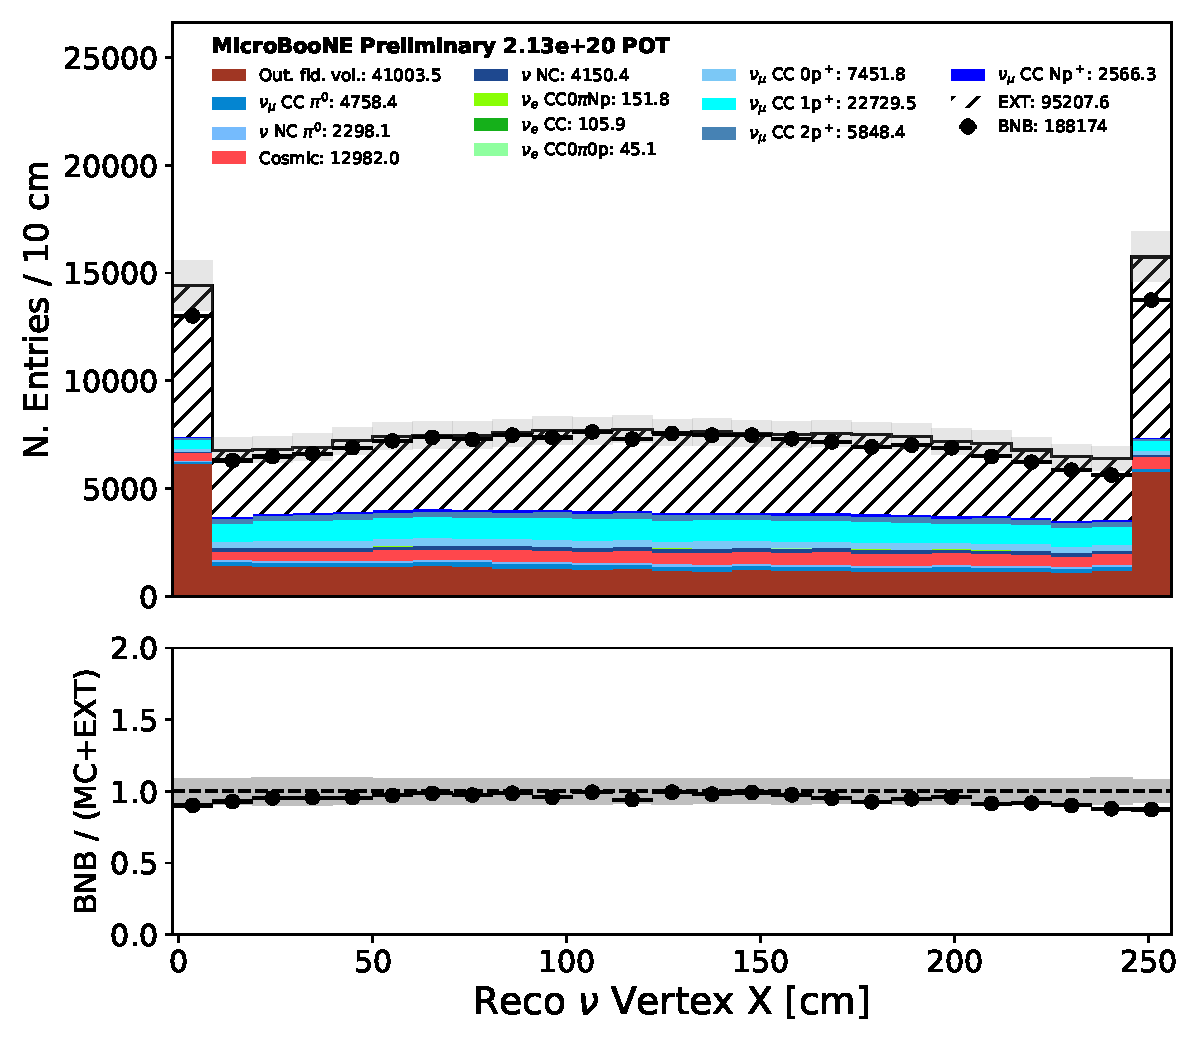
\includegraphics[width=\textwidth]{NuMuCCsel/Images/Ryan/appendix_presel_input_R3/reco_nu_vtx_sce_x_07262020_samples_event_category.pdf}
        \end{subfigure}
        %----- Y ------%
        \begin{subfigure}[b]{0.3\textwidth}
        \centering
        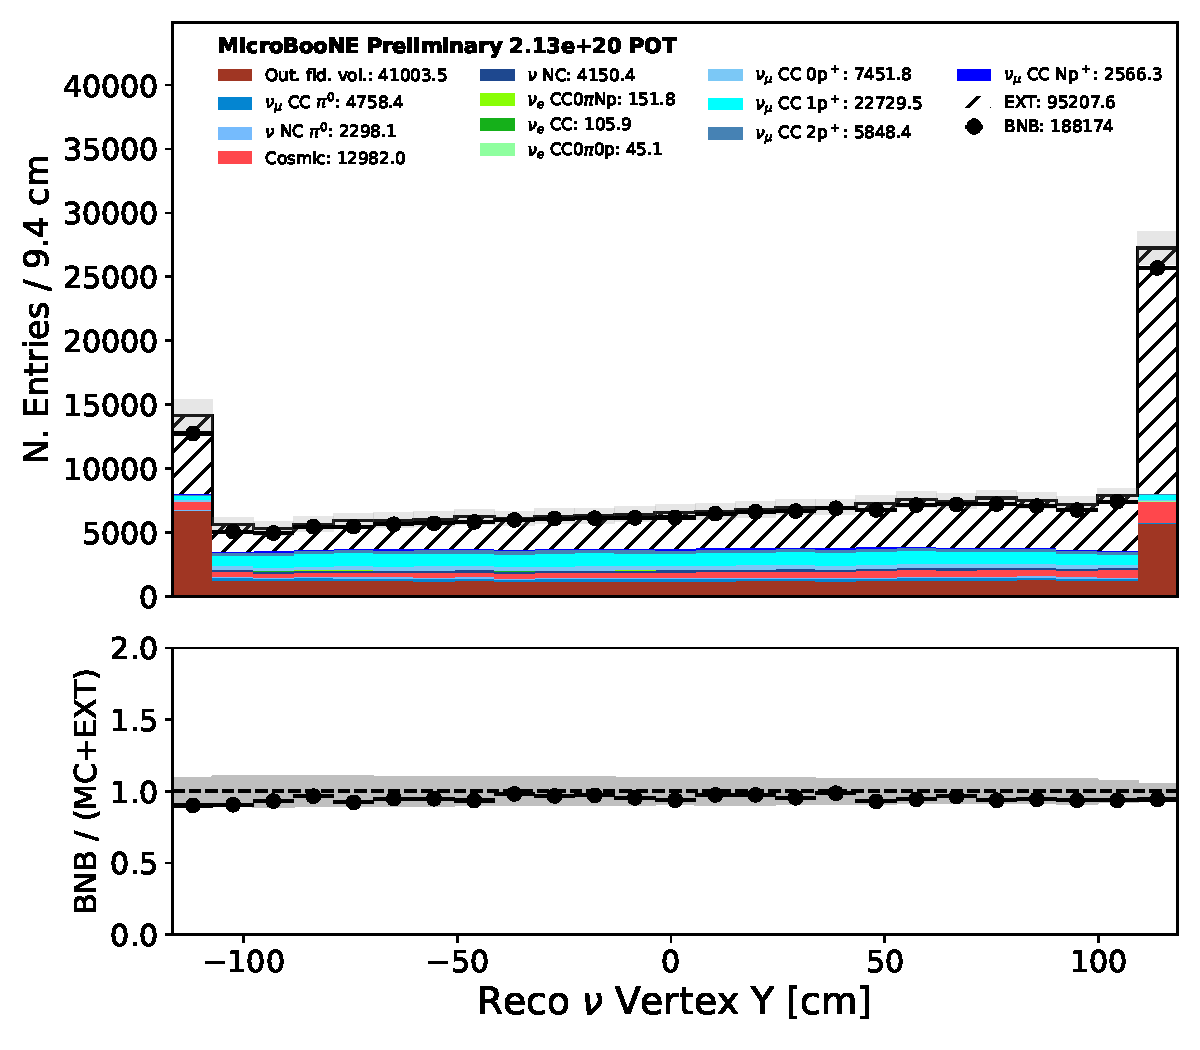
\includegraphics[width=\textwidth]{NuMuCCsel/Images/Ryan/appendix_presel_input_R3/reco_nu_vtx_sce_y_07262020_samples_event_category.pdf}
        \end{subfigure}
        %----- Z ------%
        \begin{subfigure}[b]{0.3\textwidth}
        \centering
        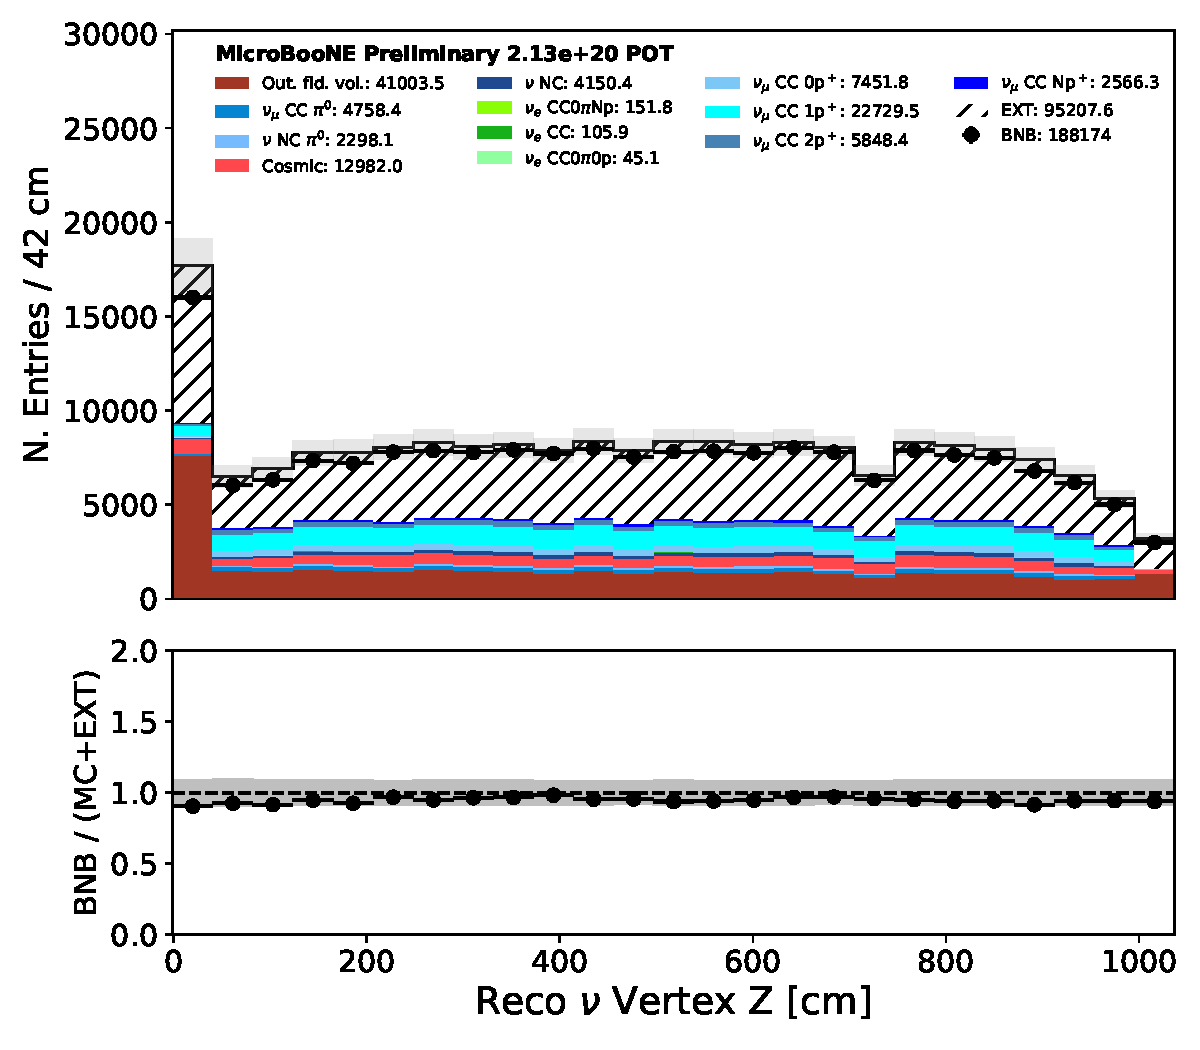
\includegraphics[width=\textwidth]{NuMuCCsel/Images/Ryan/appendix_presel_input_R3/reco_nu_vtx_sce_z_07262020_samples_event_category.pdf}
        \end{subfigure}
    \caption{Reconstructed vertex locations for all events that pass the SliceID filter.}
    \label{fig::Appendix::constraint:inputvars:reconuvtx}
\end{figure}

% ---- CRT VARS ---- %
\begin{figure}[H]
    \centering
        %-----_closest ------%
        \begin{subfigure}[b]{0.3\textwidth}
        \centering
        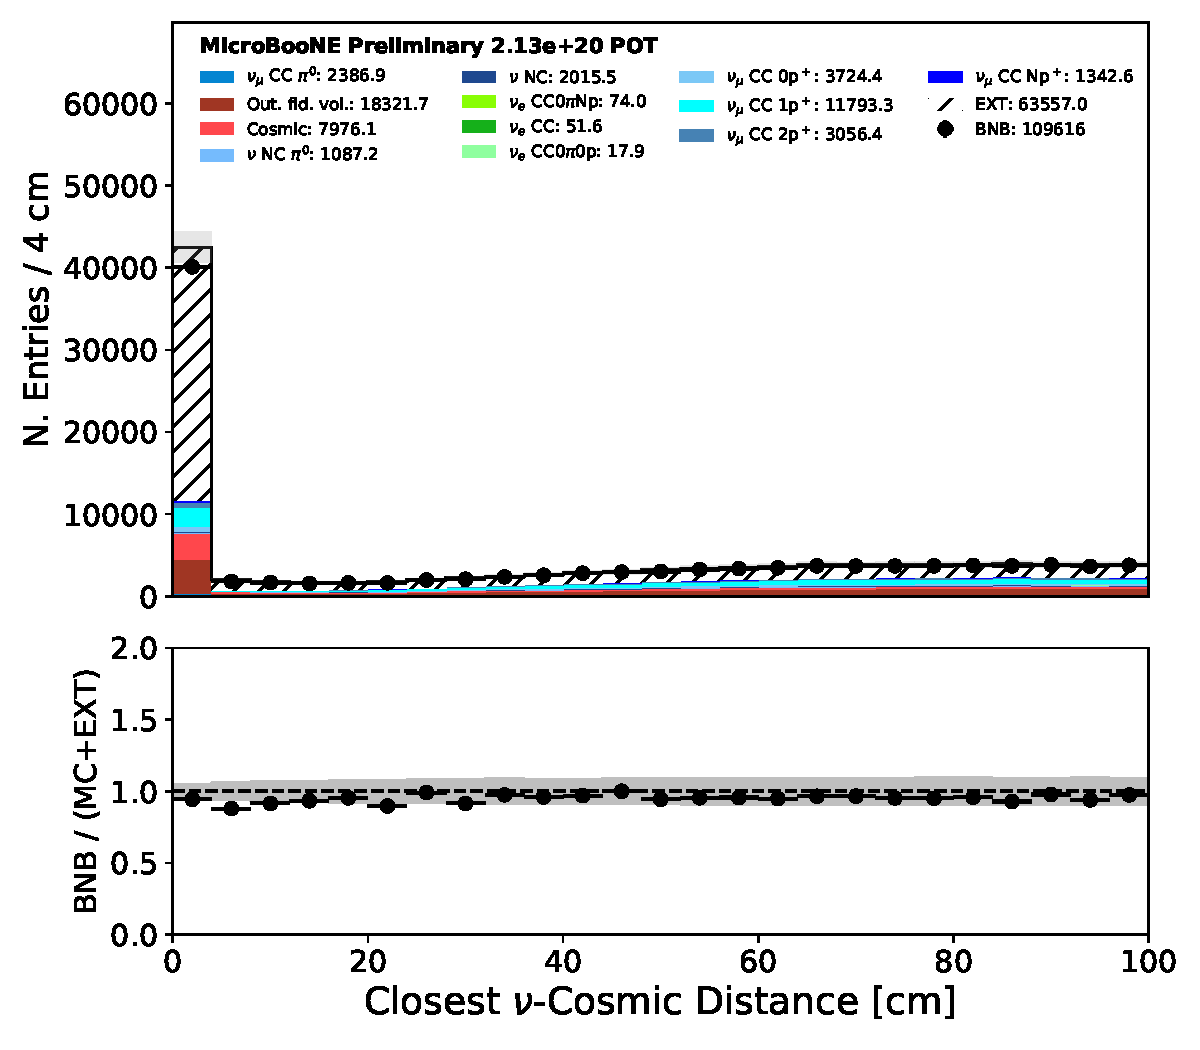
\includegraphics[width=\textwidth]{NuMuCCsel/Images/Ryan/appendix_presel_input_R3/_closestNuCosmicDist_07272020_samples_event_category.pdf}
        \end{subfigure}
        %-----CRThitPE------%
        \begin{subfigure}[b]{0.3\textwidth}
        \centering
        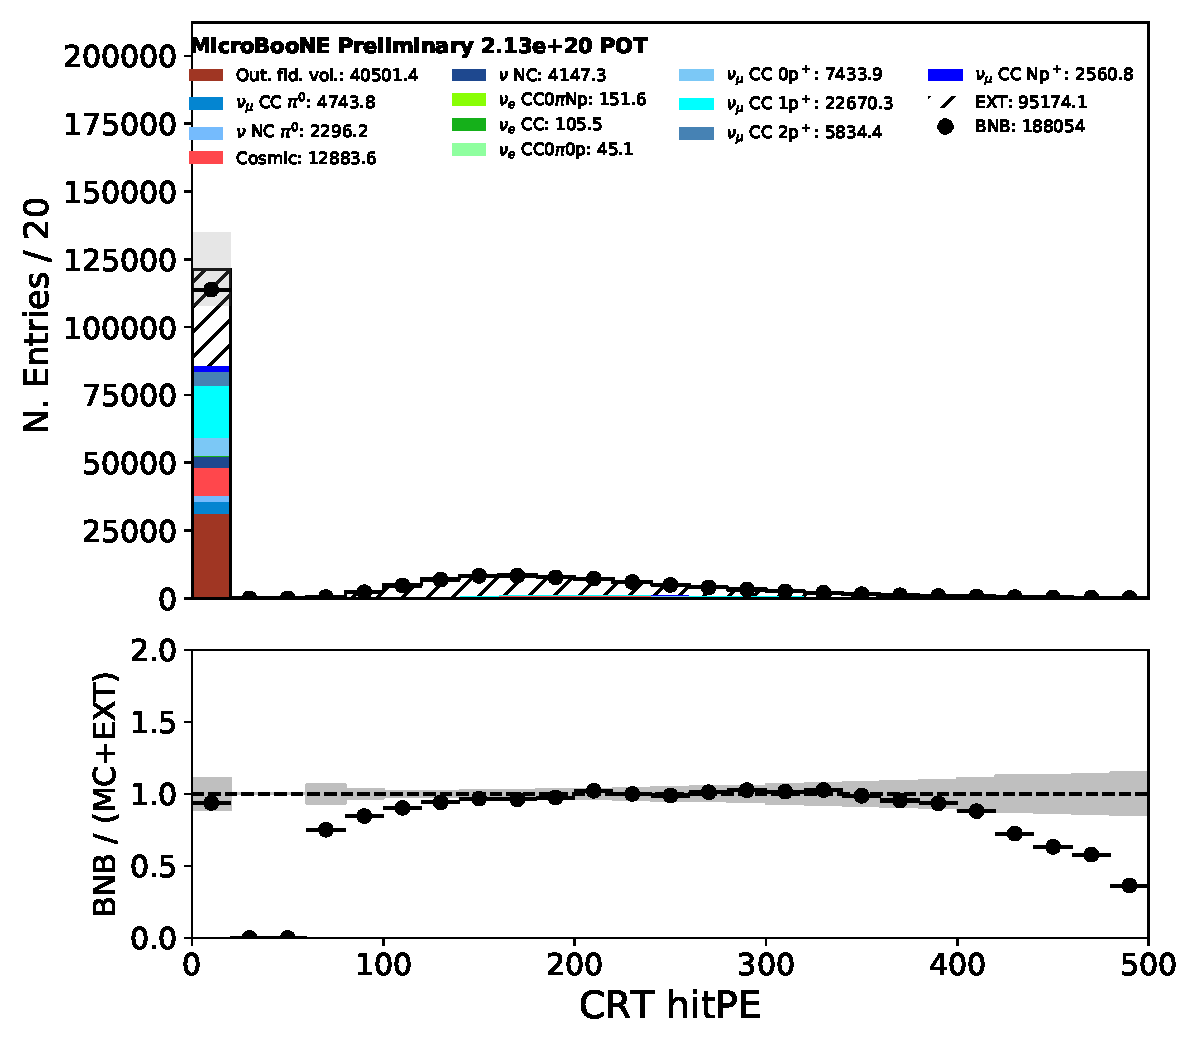
\includegraphics[width=\textwidth]{NuMuCCsel/Images/Ryan/appendix_presel_input_R3/crthitpe_07262020_samples_event_category.pdf}
        \end{subfigure}
        %-----CRTveto------%
        \begin{subfigure}[b]{0.3\textwidth}
        \centering
        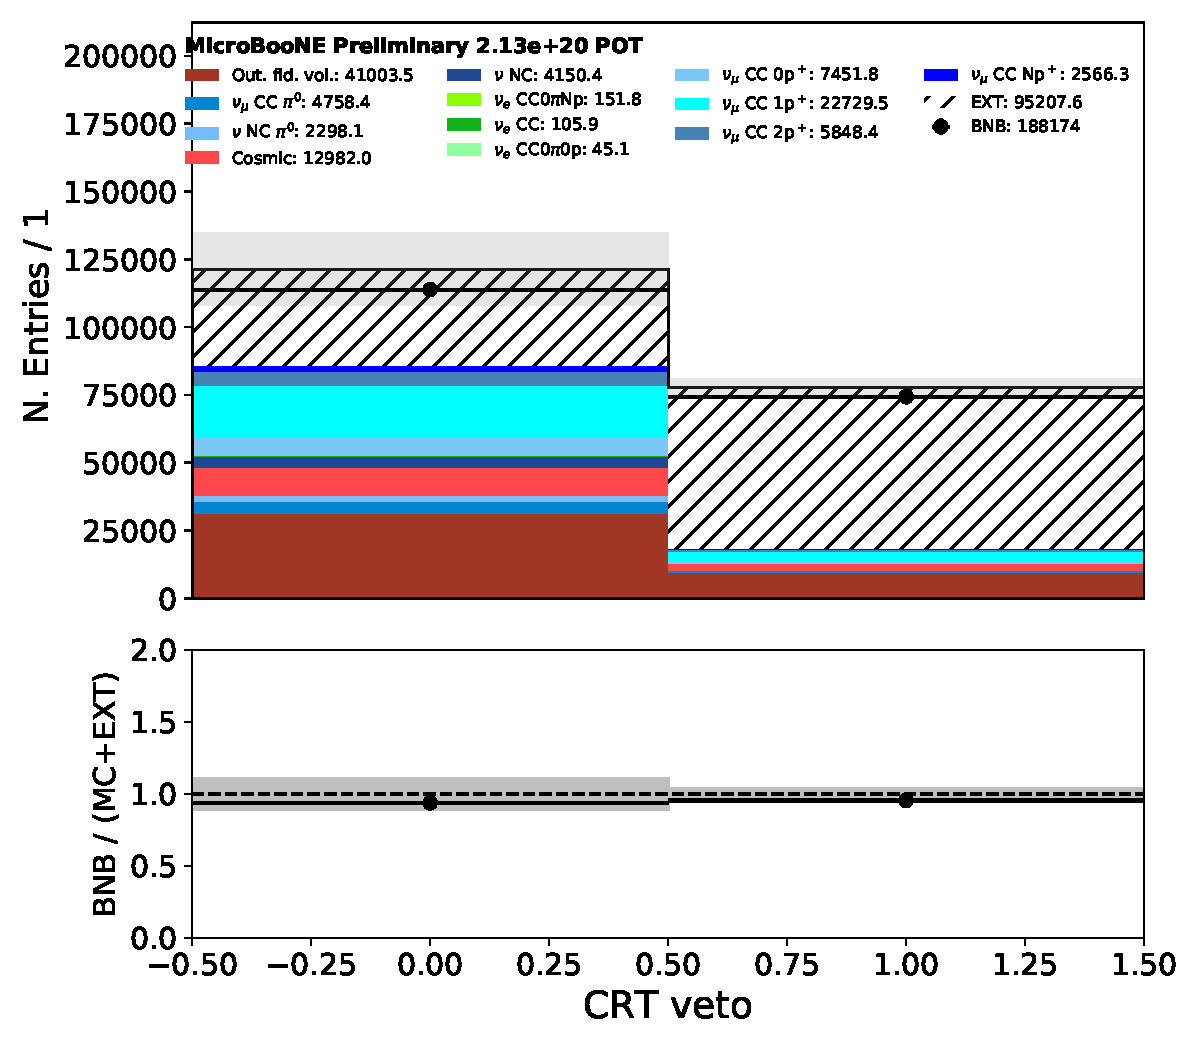
\includegraphics[width=\textwidth]{NuMuCCsel/Images/Ryan/appendix_presel_input_R3/crtveto_07262020_samples_event_category.pdf}
        \end{subfigure}
    \caption{Variables produced from the data of MicroBooNE's cosmic ray tagger. See section \ref{sec:sliceID:CRT} for more information. Only SliceID filter applied.}
    \label{fig::Appendix::constraint:inputvars:crtvars}
\end{figure}

% ---- OTHERS ---- %
\begin{figure}[H]
    \centering
        %-----CONTAINED FRAC-----%
        \begin{subfigure}[b]{0.3\textwidth}
        \centering
        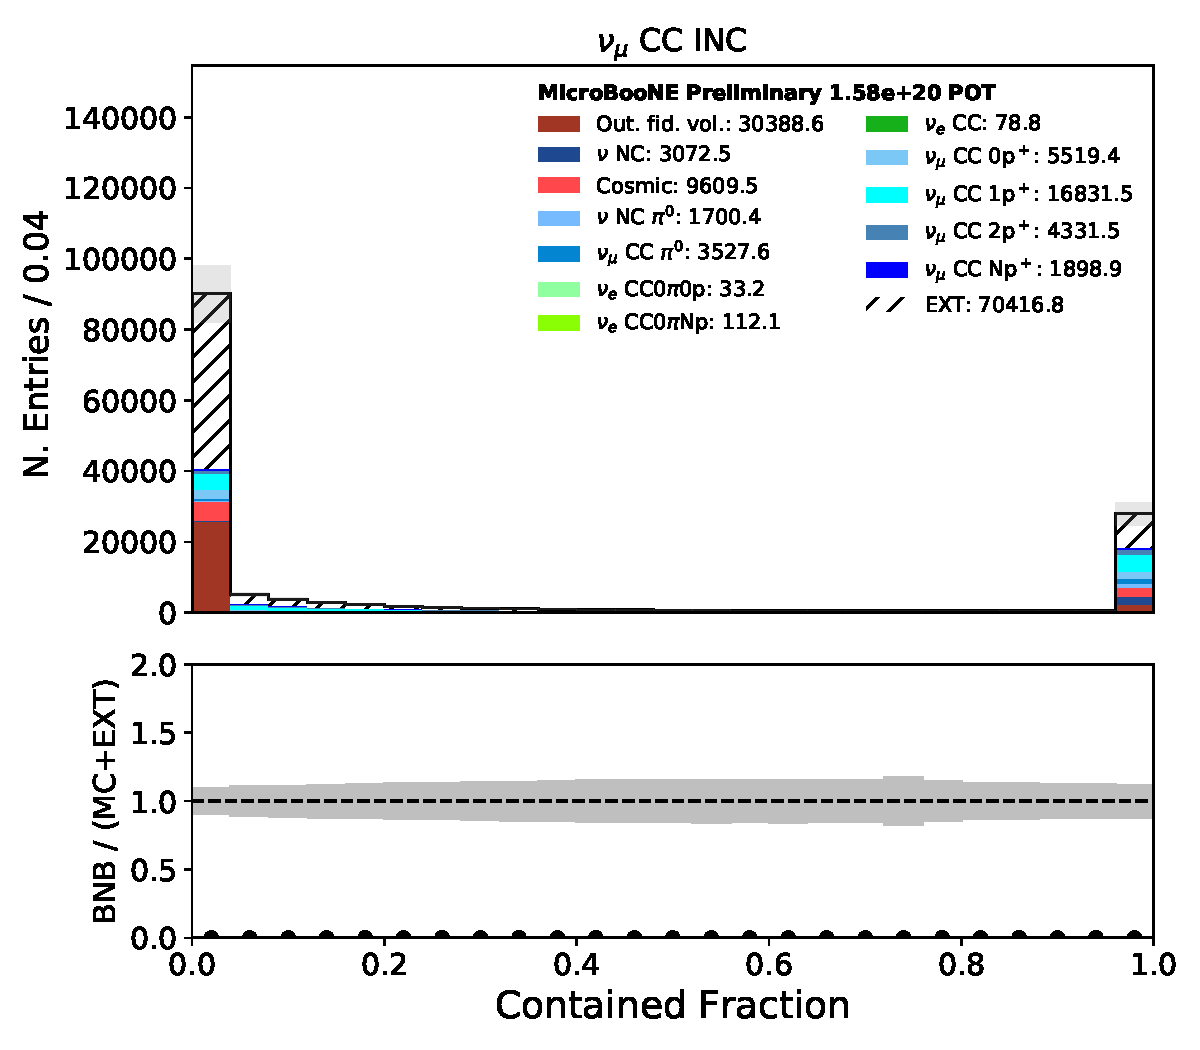
\includegraphics[width=\textwidth]{NuMuCCsel/Images/Ryan/appendix_presel_input_R3/contained_fraction_06122020_samples_G1_longest_detsys_event_category.pdf}
        \end{subfigure}
        %-----TOPOSCORE------%
        \begin{subfigure}[b]{0.3\textwidth}
        \centering
        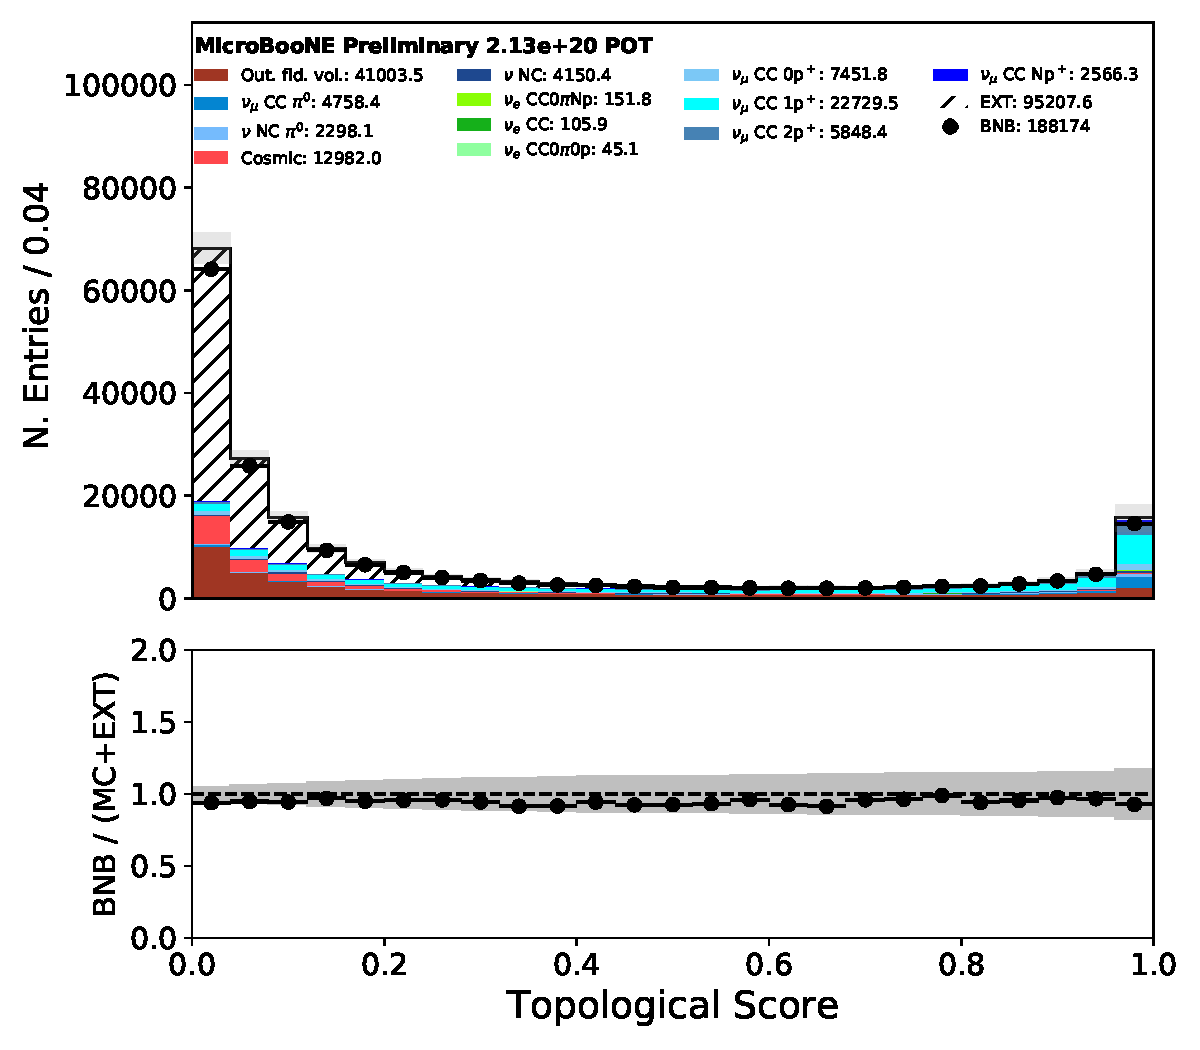
\includegraphics[width=\textwidth]{NuMuCCsel/Images/Ryan/appendix_presel_input_R3/topological_score_07262020_samples_event_category.pdf}
        \end{subfigure}
    \caption{Other variables relevant to the preselection. Contained fraction describes what fraction of each event is within the fiducial volume. The topological score is a machine-learned quantity that uses the topology of the event to discriminate between cosmic and signal dominated events. Only SliceID filter applied.}
    \label{fig::Appendix::constraint:inputvars:others}
\end{figure}

\subsection{Muon Selection Input}
\label{ssec:Appendix:numu:muonselinput}
% ---- STARTPOINT ---- %
\begin{figure}[H]
    \centering
        %----- X ------%
        \begin{subfigure}[b]{0.3\textwidth}
        \centering
        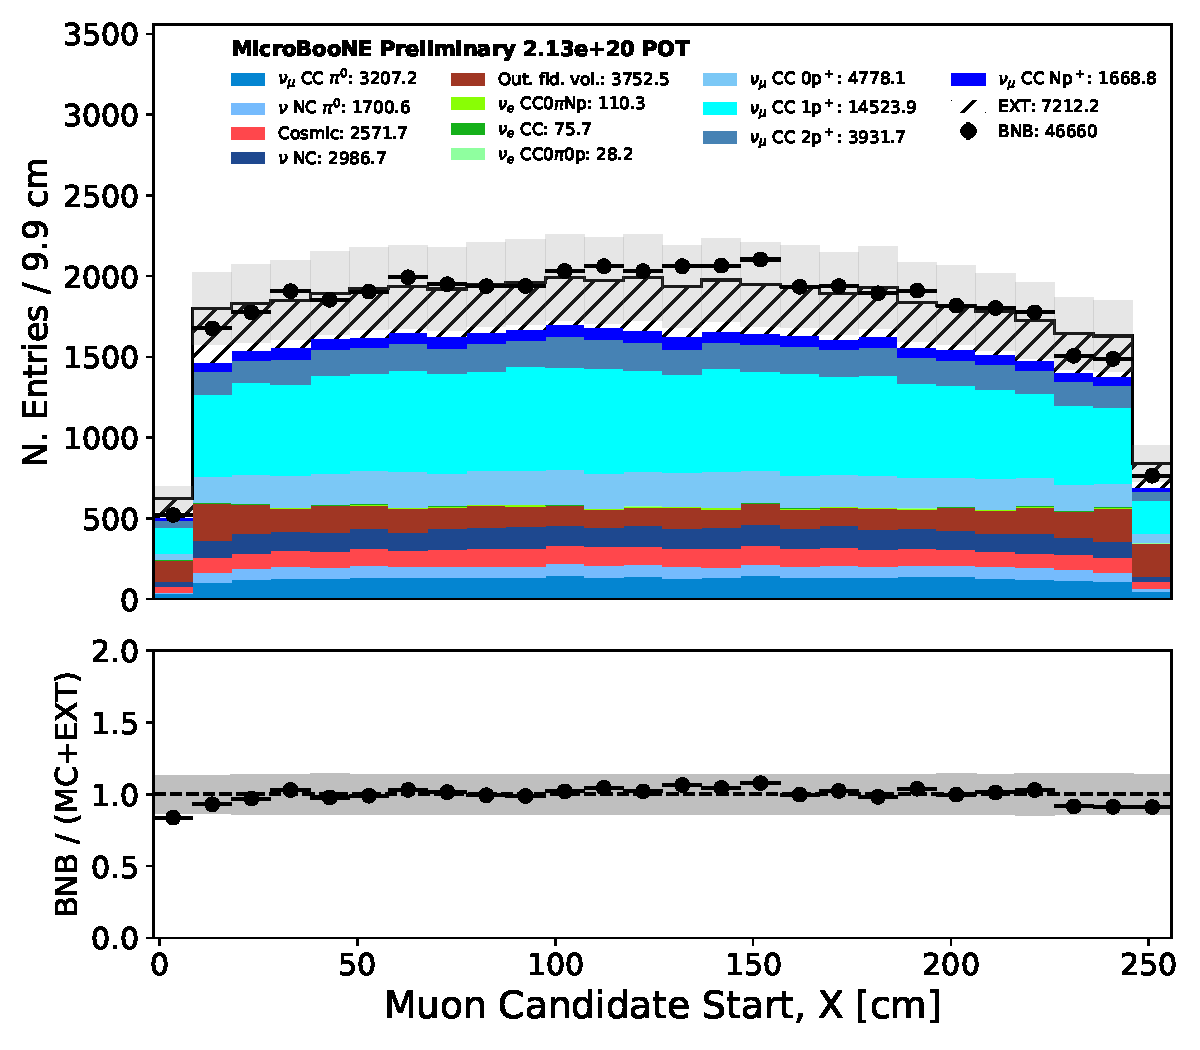
\includegraphics[width=\textwidth]{NuMuCCsel/Images/Ryan/appendix_muonsel_input_R3/trk_sce_start_x_v_07232020_presel_samples_detsys_event_category.pdf}
        \end{subfigure}
        %----- Y ------%
        \begin{subfigure}[b]{0.3\textwidth}
        \centering
        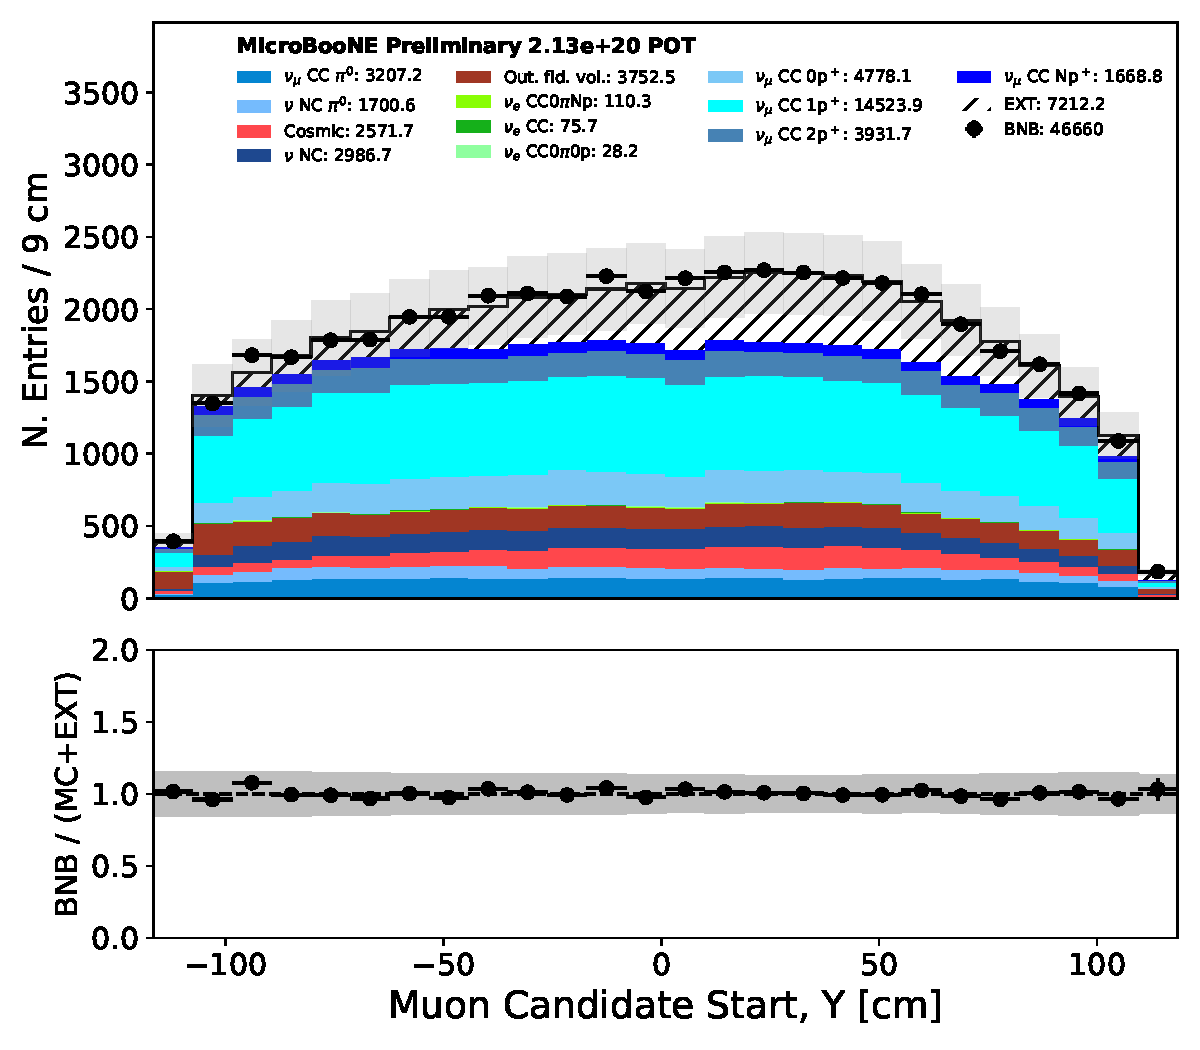
\includegraphics[width=\textwidth]{NuMuCCsel/Images/Ryan/appendix_muonsel_input_R3/trk_sce_start_y_v_07232020_presel_samples_detsys_event_category.pdf}
        \end{subfigure}
        %----- Z ------%
        \begin{subfigure}[b]{0.3\textwidth}
        \centering
        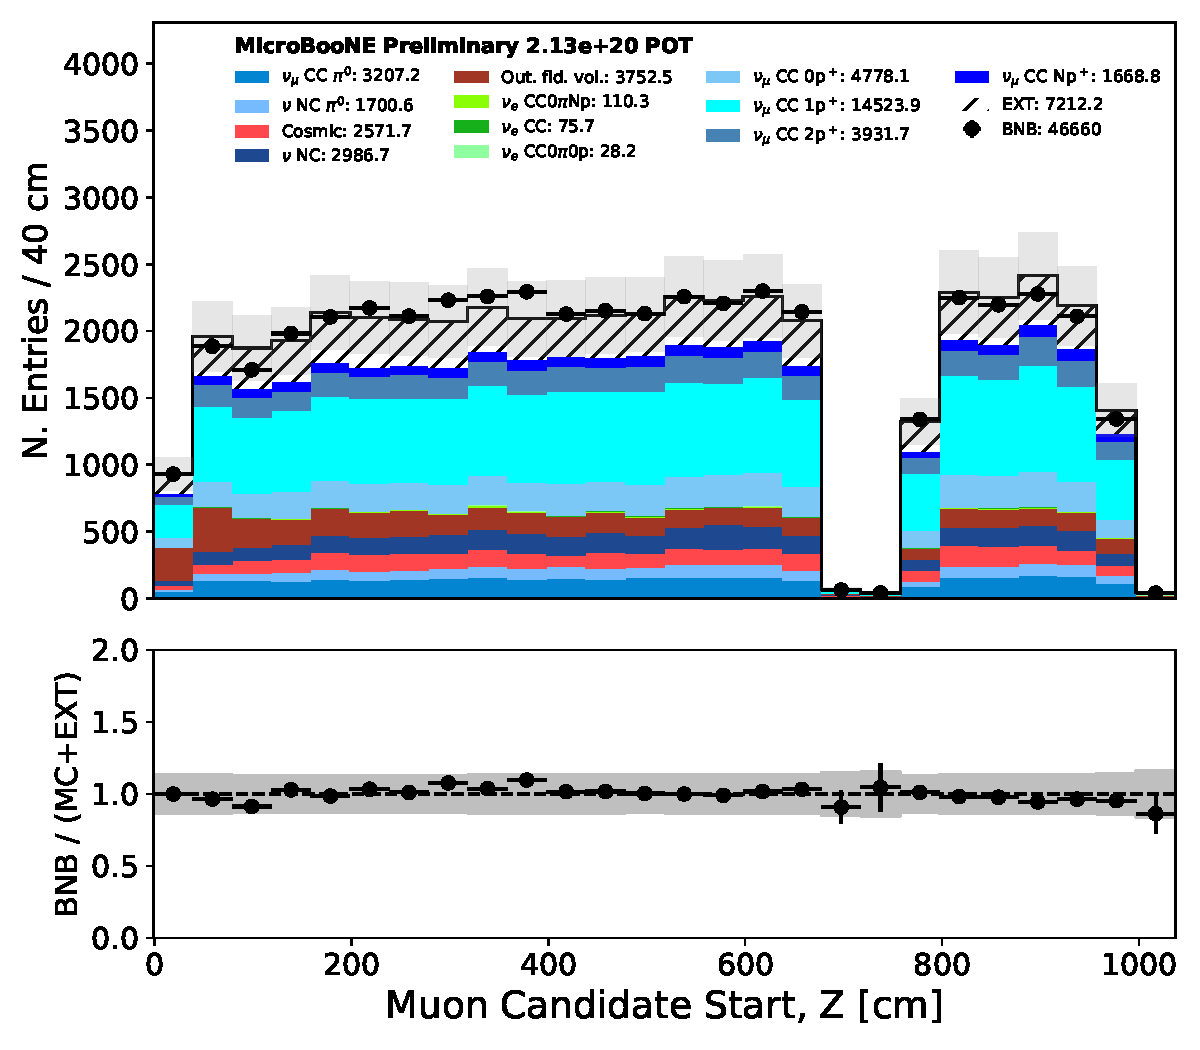
\includegraphics[width=\textwidth]{NuMuCCsel/Images/Ryan/appendix_muonsel_input_R3/trk_sce_start_z_v_07232020_presel_samples_detsys_event_category.pdf}
        \end{subfigure}
    \caption{Reconstructed \textbf{start}-points for longest track in each event passing preselection. Used to select contained muons. Preselection applied.}
    \label{fig::Appendix::constraint:inputvars:startpoints}
\end{figure}

% ---- ENDPOINT ---- %
\begin{figure}[H]
    \centering
        %----- X ------%
        \begin{subfigure}[b]{0.3\textwidth}
        \centering
        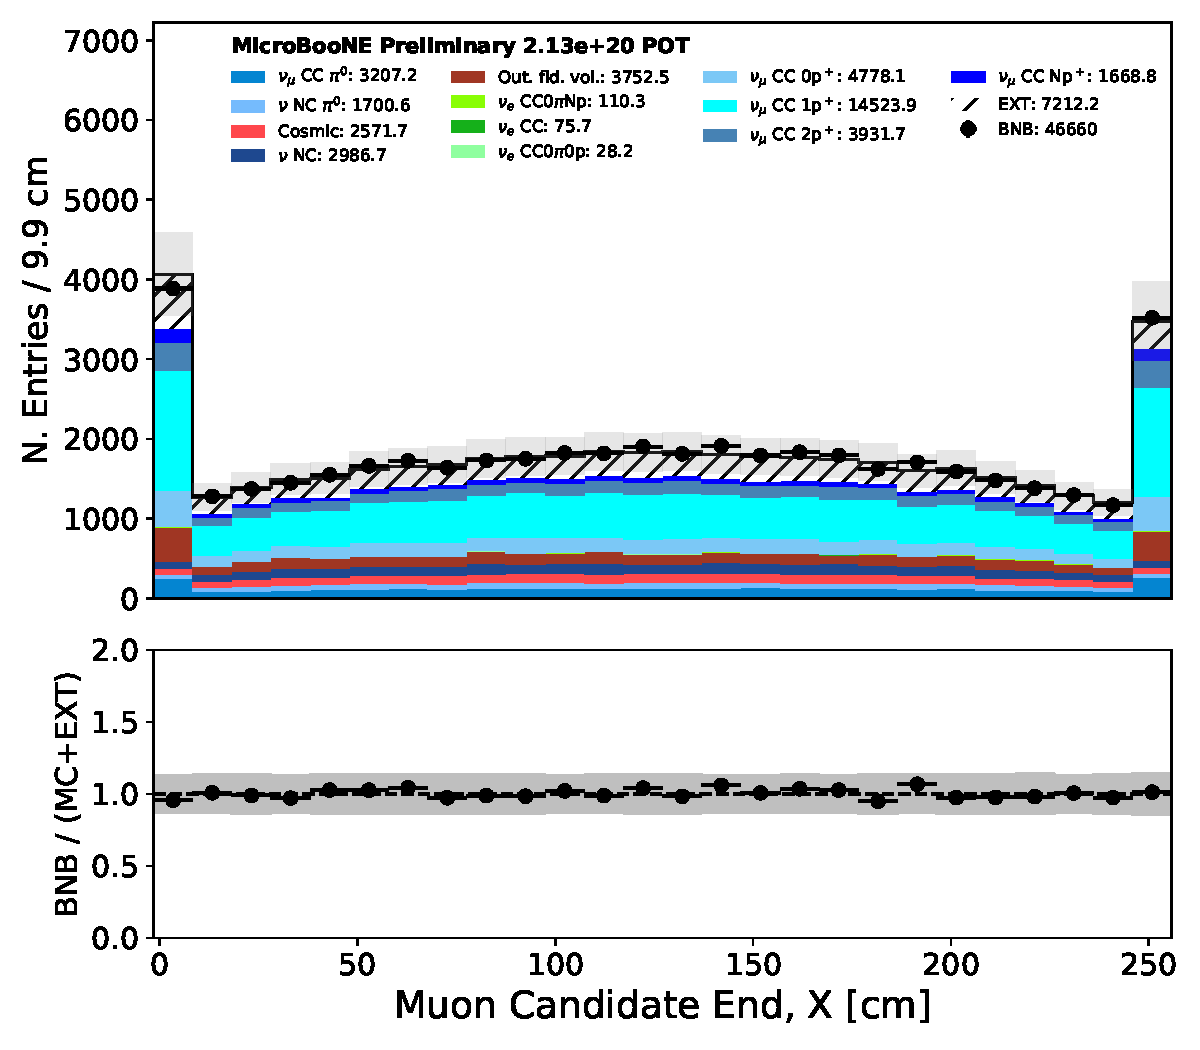
\includegraphics[width=\textwidth]{NuMuCCsel/Images/Ryan/appendix_muonsel_input_R3/trk_sce_end_x_v_07232020_presel_samples_detsys_event_category.pdf}
        \end{subfigure}
        %----- Y ------%
        \begin{subfigure}[b]{0.3\textwidth}
        \centering
        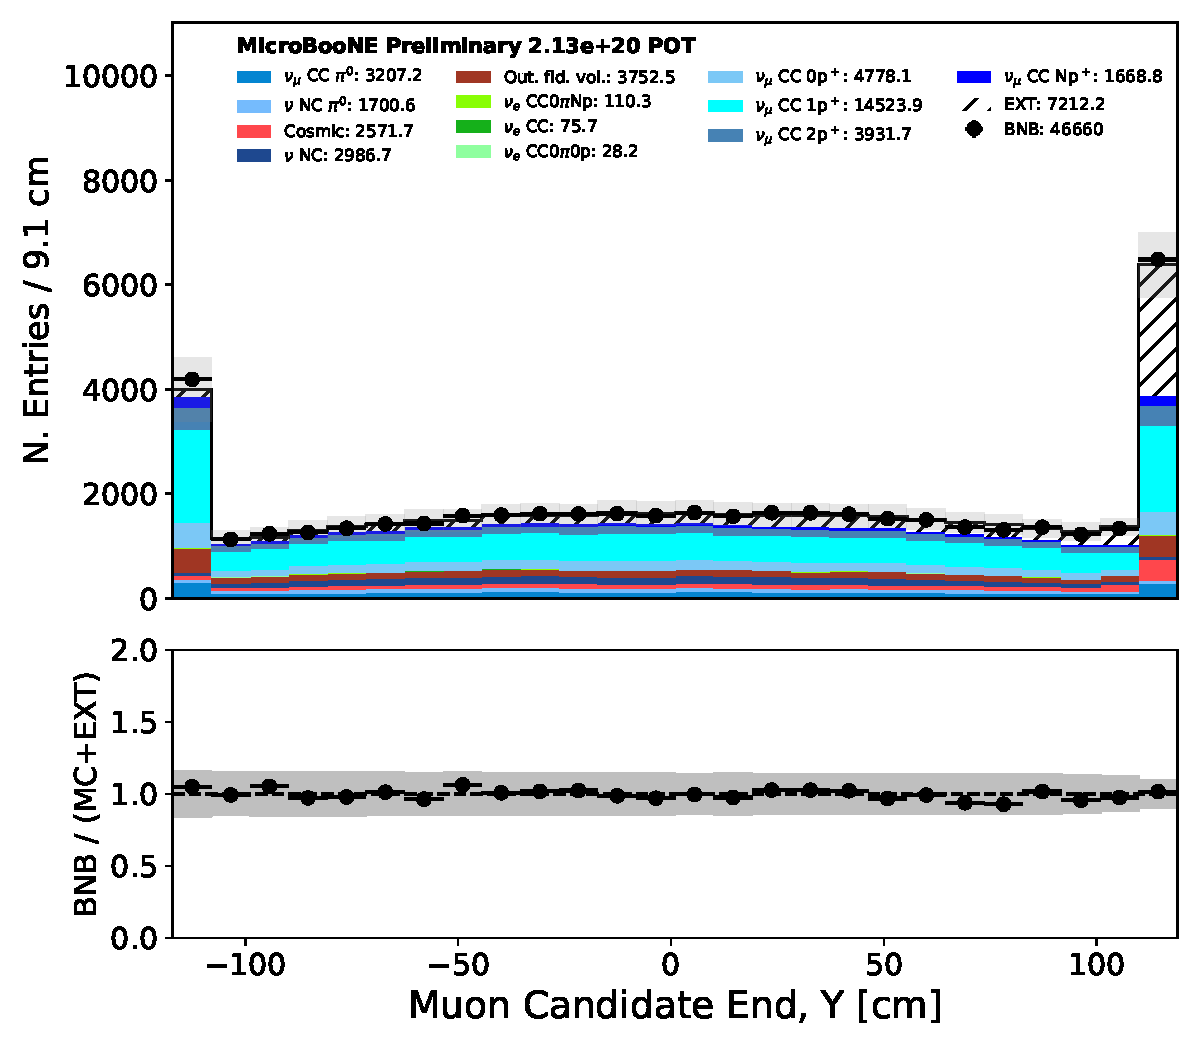
\includegraphics[width=\textwidth]{NuMuCCsel/Images/Ryan/appendix_muonsel_input_R3/trk_sce_end_y_v_07232020_presel_samples_detsys_event_category.pdf}
        \end{subfigure}
        %----- Z ------%
        \begin{subfigure}[b]{0.3\textwidth}
        \centering
        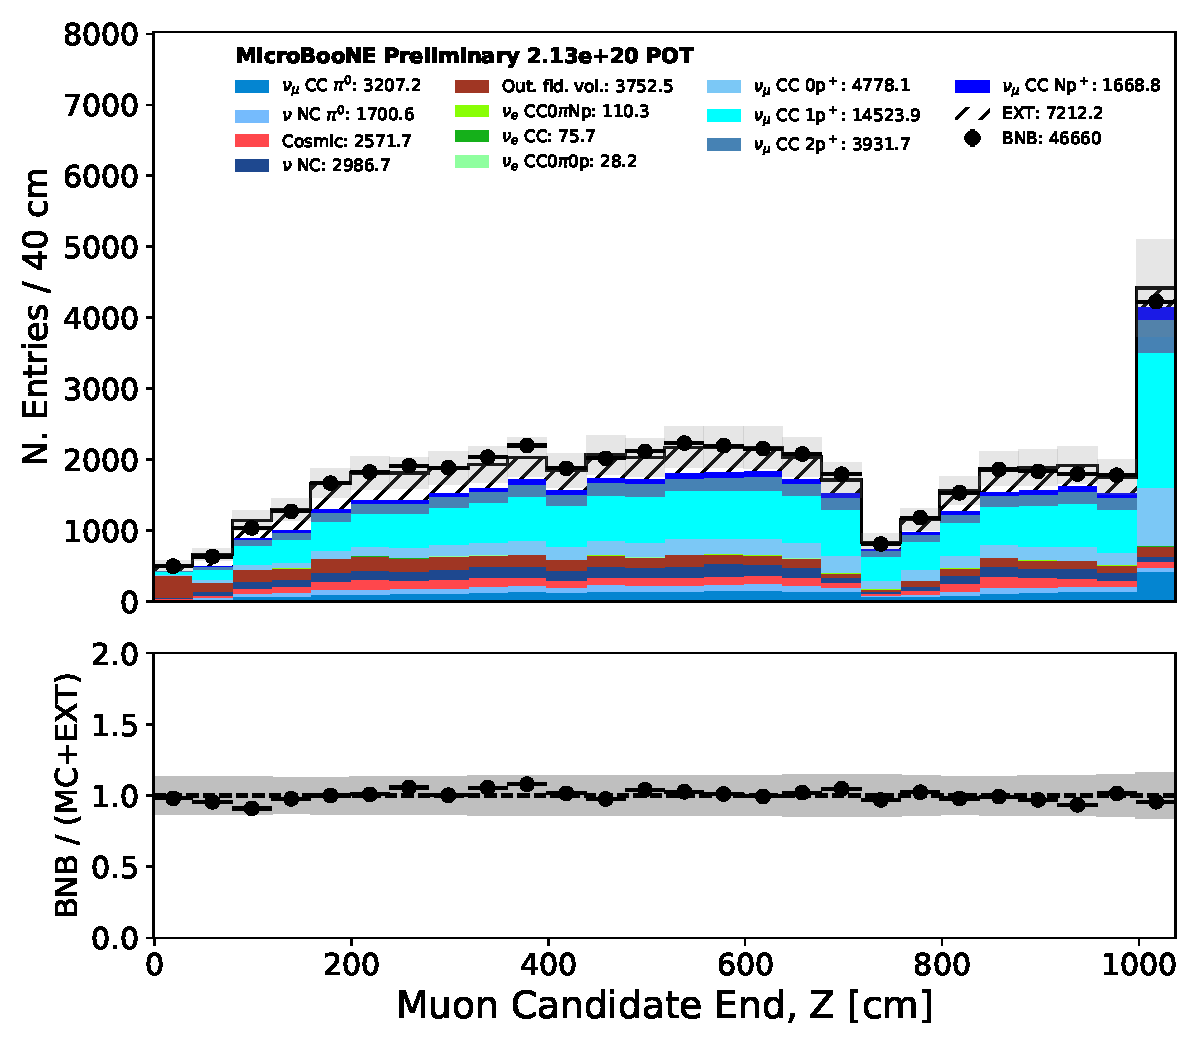
\includegraphics[width=\textwidth]{NuMuCCsel/Images/Ryan/appendix_muonsel_input_R3/trk_sce_end_z_v_07232020_presel_samples_detsys_event_category.pdf}
        \end{subfigure}
    \caption{Reconstructed \textbf{end}-points for longest track in each event passing preselection. Used to select contained muons. Preselection applied}
    \label{fig::Appendix::constraint:inputvars:endpoints}
\end{figure}

%-------- SCORES --------%
\begin{figure}[H]
    \centering
        %----- X ------%
        \begin{subfigure}[b]{0.3\textwidth}
        \centering
        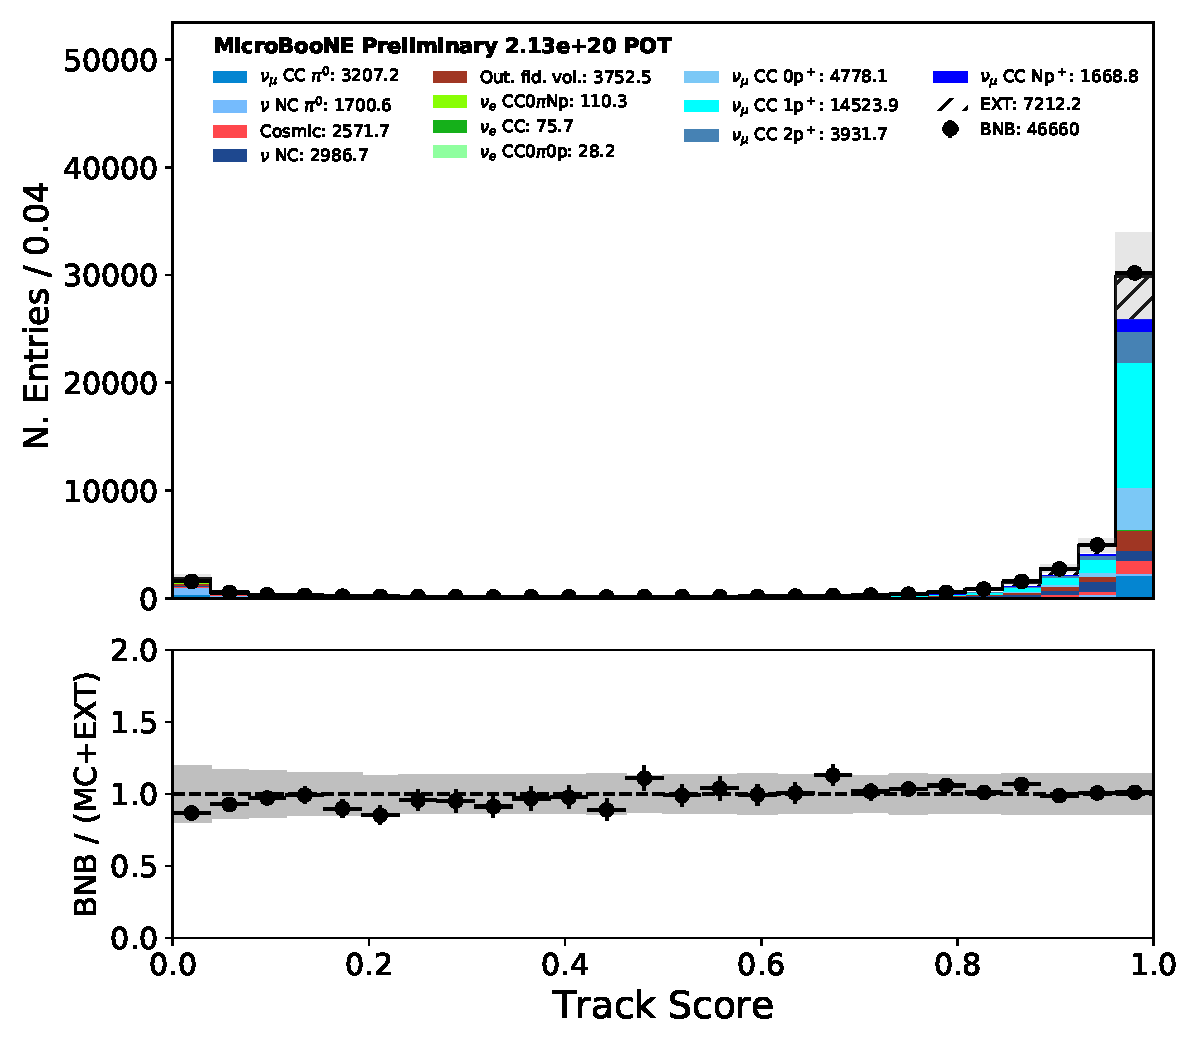
\includegraphics[width=\textwidth]{NuMuCCsel/Images/Ryan/appendix_muonsel_input_R3/trk_score_v_07232020_presel_samples_detsys_event_category.pdf}
        \end{subfigure}
        %----- Y ------%
        \begin{subfigure}[b]{0.3\textwidth}
        \centering
        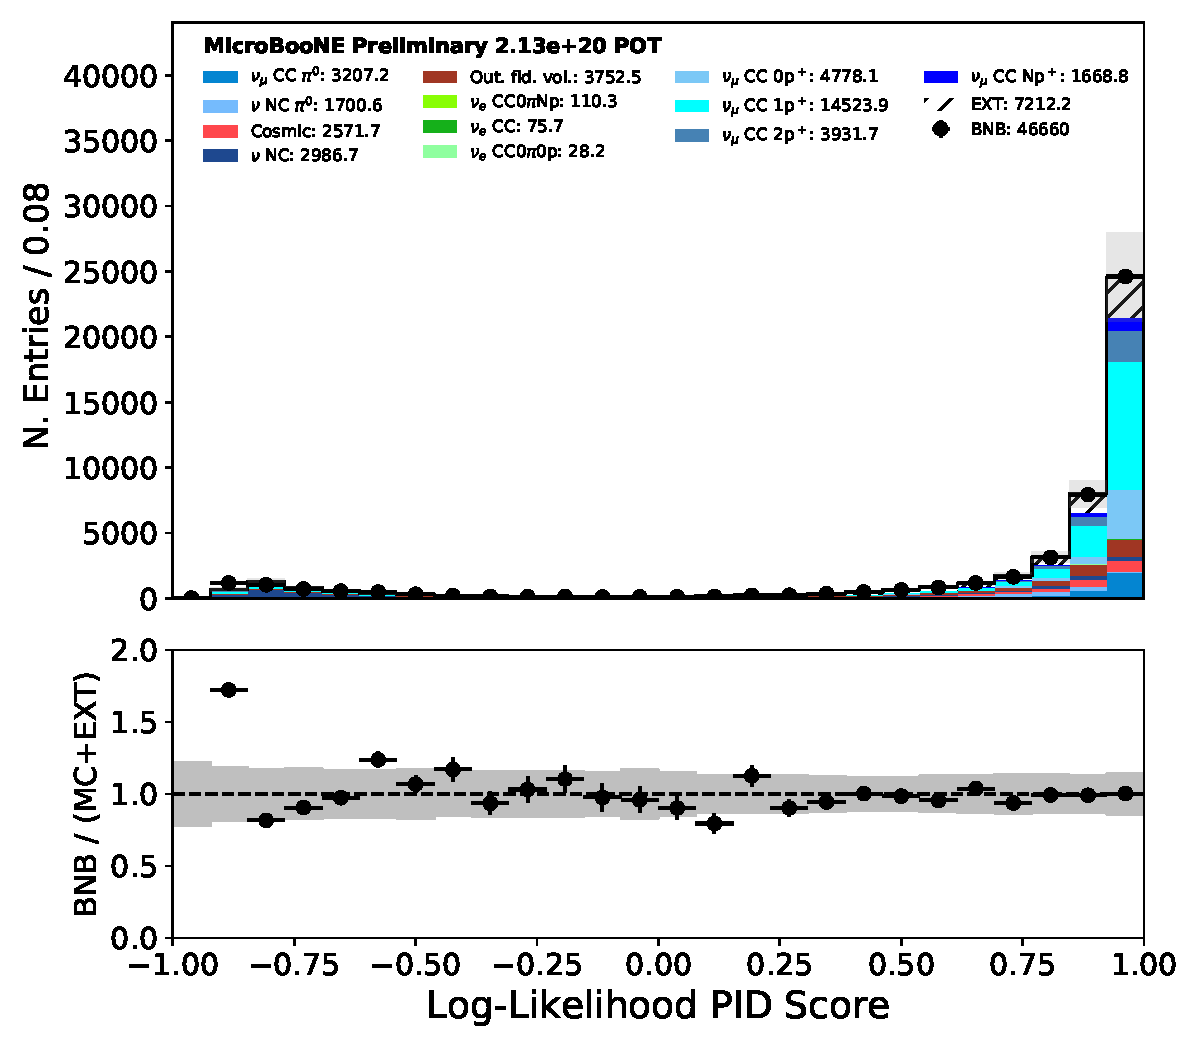
\includegraphics[width=\textwidth]{NuMuCCsel/Images/Ryan/appendix_muonsel_input_R3/trk_llr_pid_score_v_07232020_presel_samples_detsys_event_category.pdf}
        \end{subfigure}
        %----- Z ------%
        \begin{subfigure}[b]{0.3\textwidth}
        \centering
        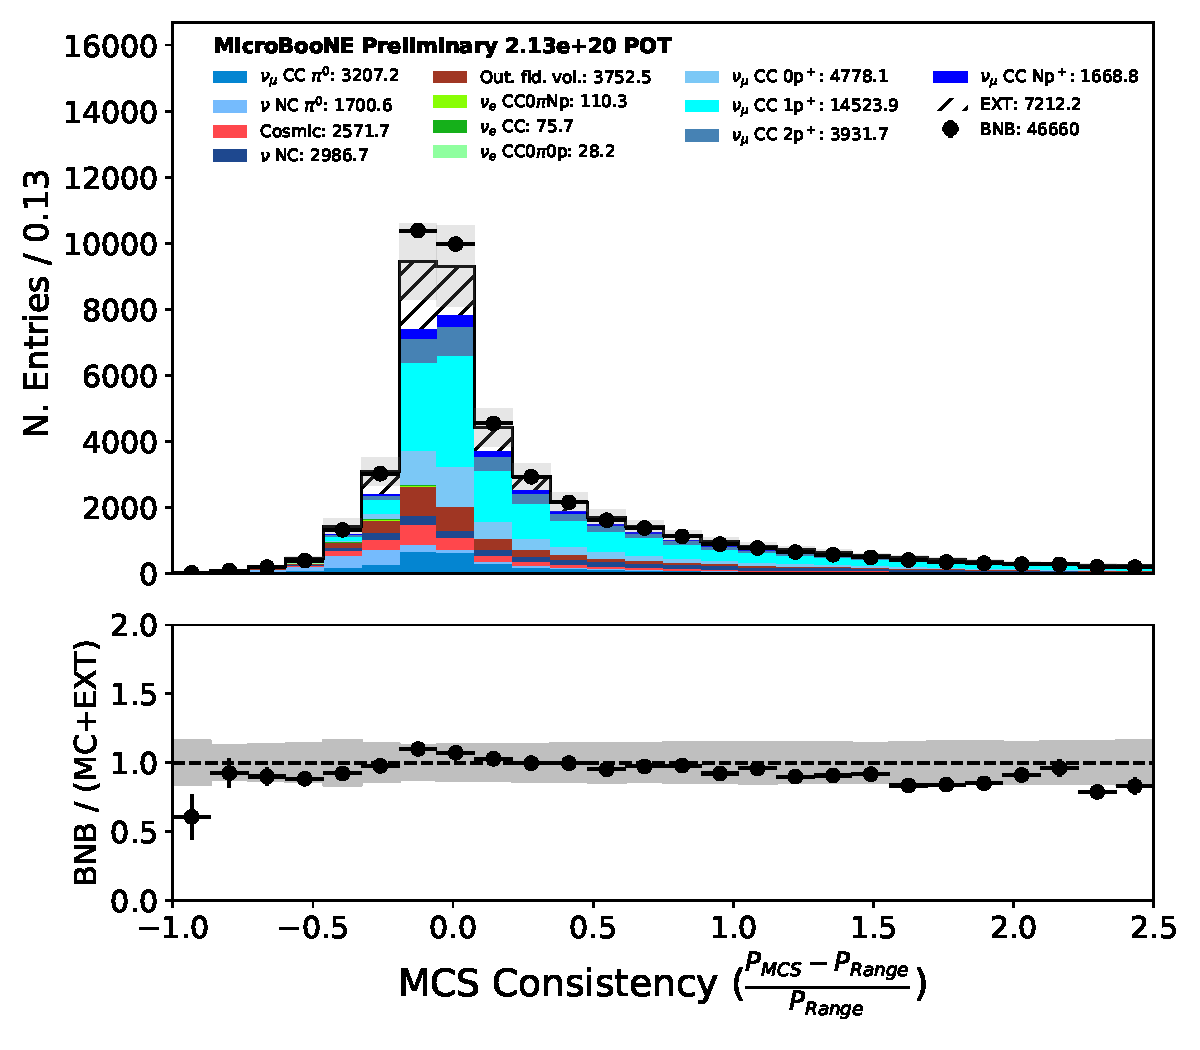
\includegraphics[width=\textwidth]{NuMuCCsel/Images/Ryan/appendix_muonsel_input_R3/trk_p_quality_v_07232020_presel_samples_detsys_event_category.pdf}
        \end{subfigure}
    \caption{Various ``scores'' assigned to each track. Preselection applied.}
    \label{fig::Appendix::constraint:inputvars:scores}
\end{figure}

%-------- Other --------%
\begin{figure}[H]
    \centering
        %----- X ------%
        \begin{subfigure}[b]{0.3\textwidth}
        \centering
        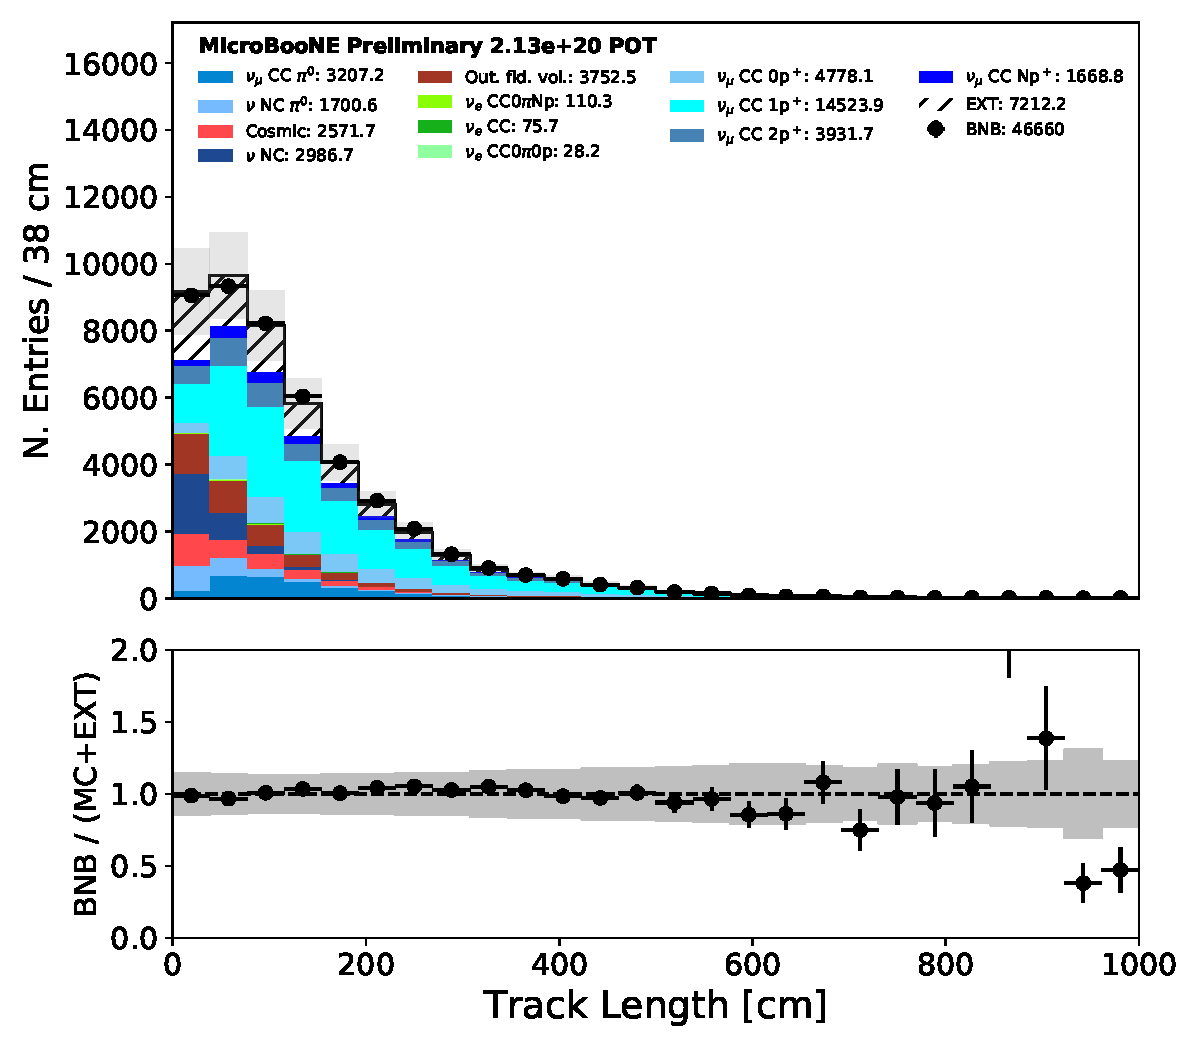
\includegraphics[width=\textwidth]{NuMuCCsel/Images/Ryan/appendix_muonsel_input_R3/trk_len_v_07232020_presel_samples_detsys_event_category.pdf}
        \end{subfigure}
        %----- Y ------%
        \begin{subfigure}[b]{0.3\textwidth}
        \centering
        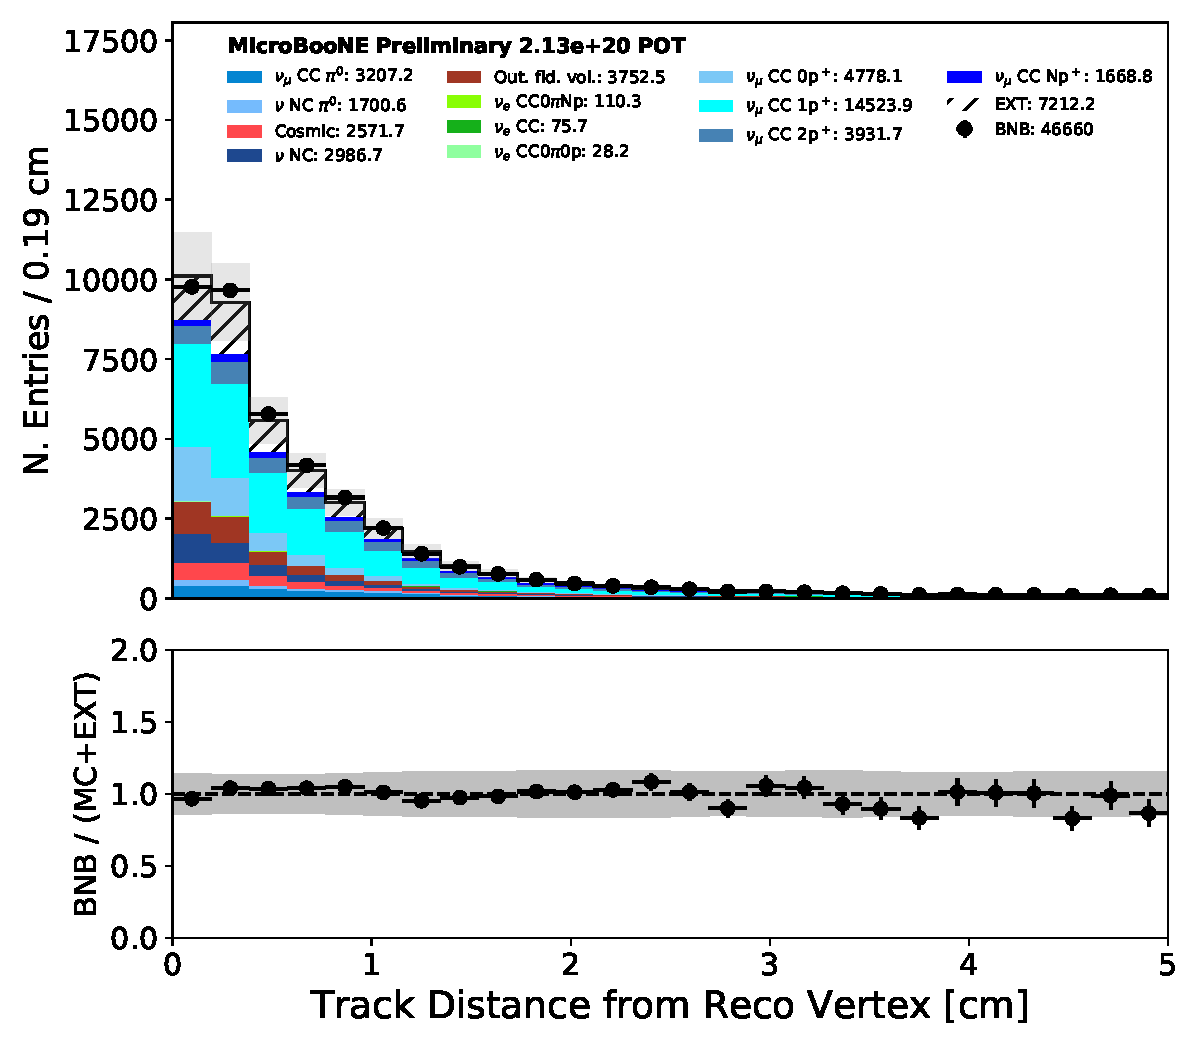
\includegraphics[width=\textwidth]{NuMuCCsel/Images/Ryan/appendix_muonsel_input_R3/trk_distance_v_07232020_presel_samples_detsys_event_category.pdf}
        \end{subfigure}
        %----- Z ------%
        \begin{subfigure}[b]{0.3\textwidth}
        \centering
        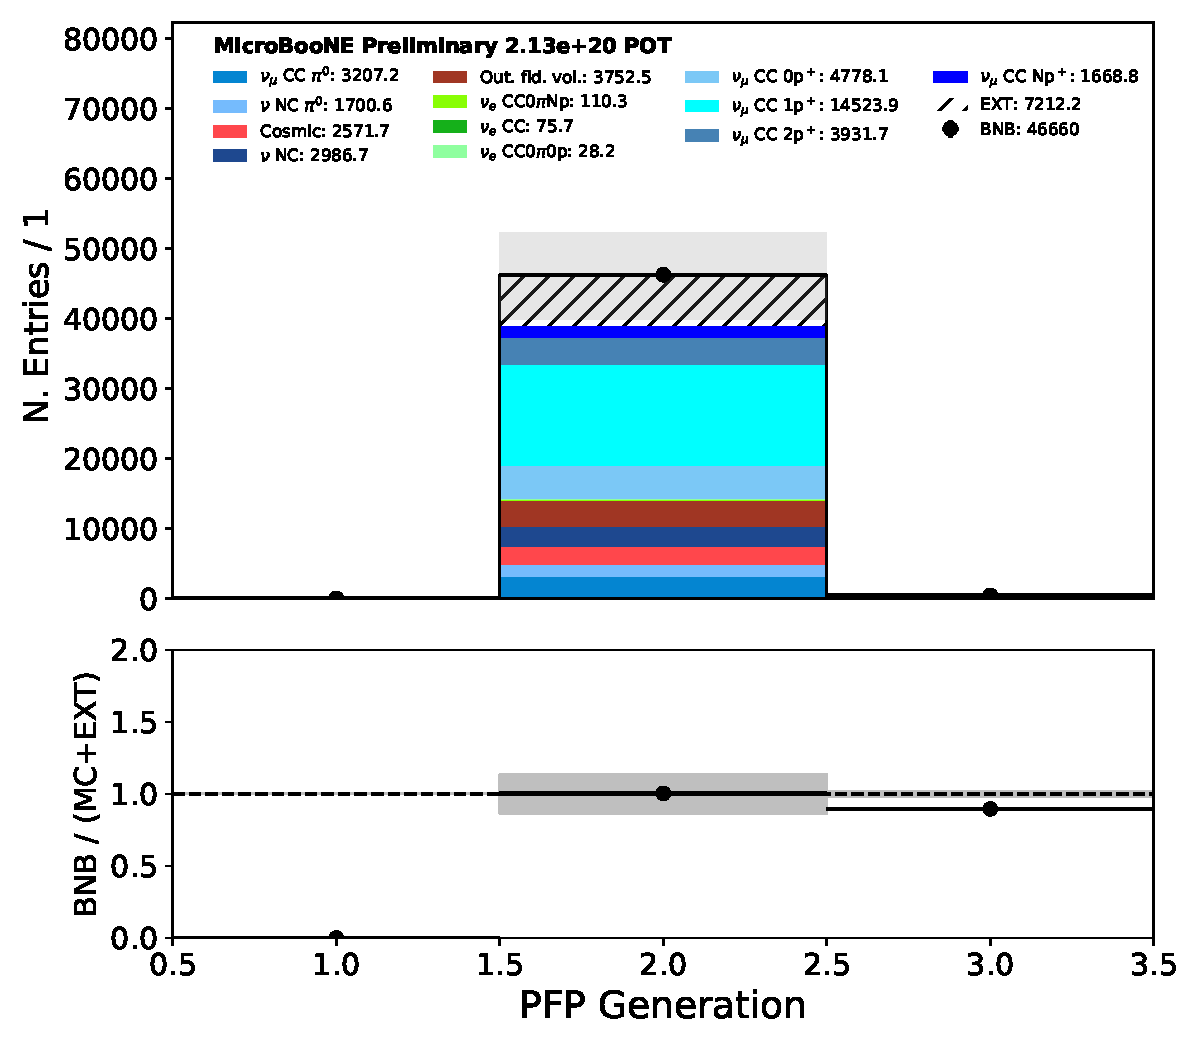
\includegraphics[width=\textwidth]{NuMuCCsel/Images/Ryan/appendix_muonsel_input_R3/pfp_generation_v_07232020_presel_samples_detsys_event_category.pdf}
        \end{subfigure}
    \caption{All other variables cut on in this selection. See section for discussion of variables. Preselection applied.}
    \label{fig::Appendix::constraint:inputvars:others}
\end{figure}

\subsection{CRT Impact}
\label{ssec:Appendix:numu:CRTimpact}
%----------CRT IMPACT-----------%
\begin{figure}[H] 
\begin{center}
    \begin{subfigure}[b]{0.35\textwidth}
        \centering
        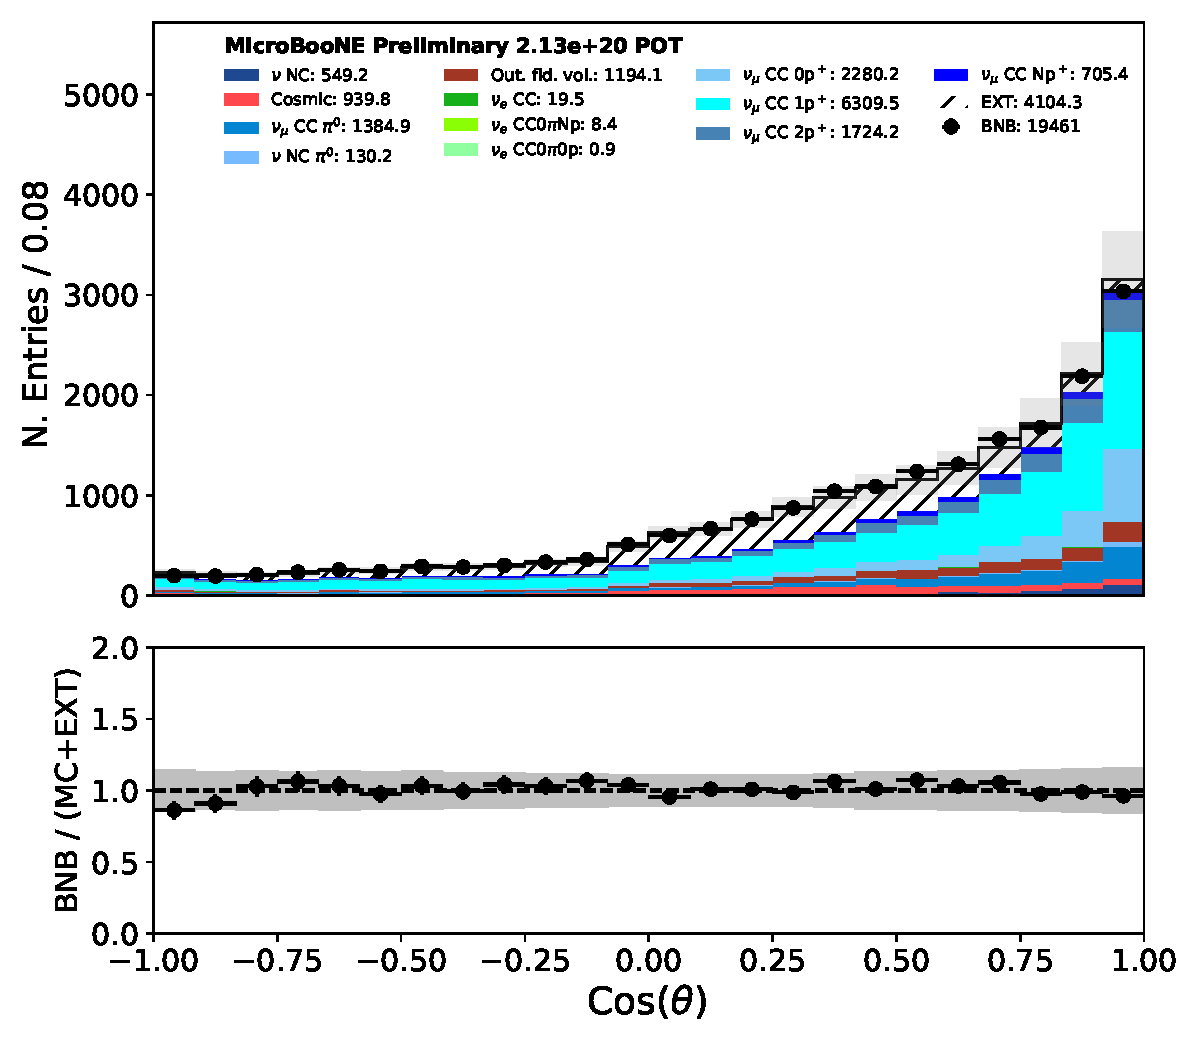
\includegraphics[width=1.00\textwidth]{NuMuCCsel/Images/Ryan/Run3_nocrt/trk_cos_theta_08052020_fullsel_samples_event_category_noCRT.pdf}
        \caption{No CRT cuts.}
        \label{fig:NuMUCCsel:ryan:run3_costheta_withCRT}
    \end{subfigure}
    \begin{subfigure}[b]{0.35\textwidth}
        \centering
        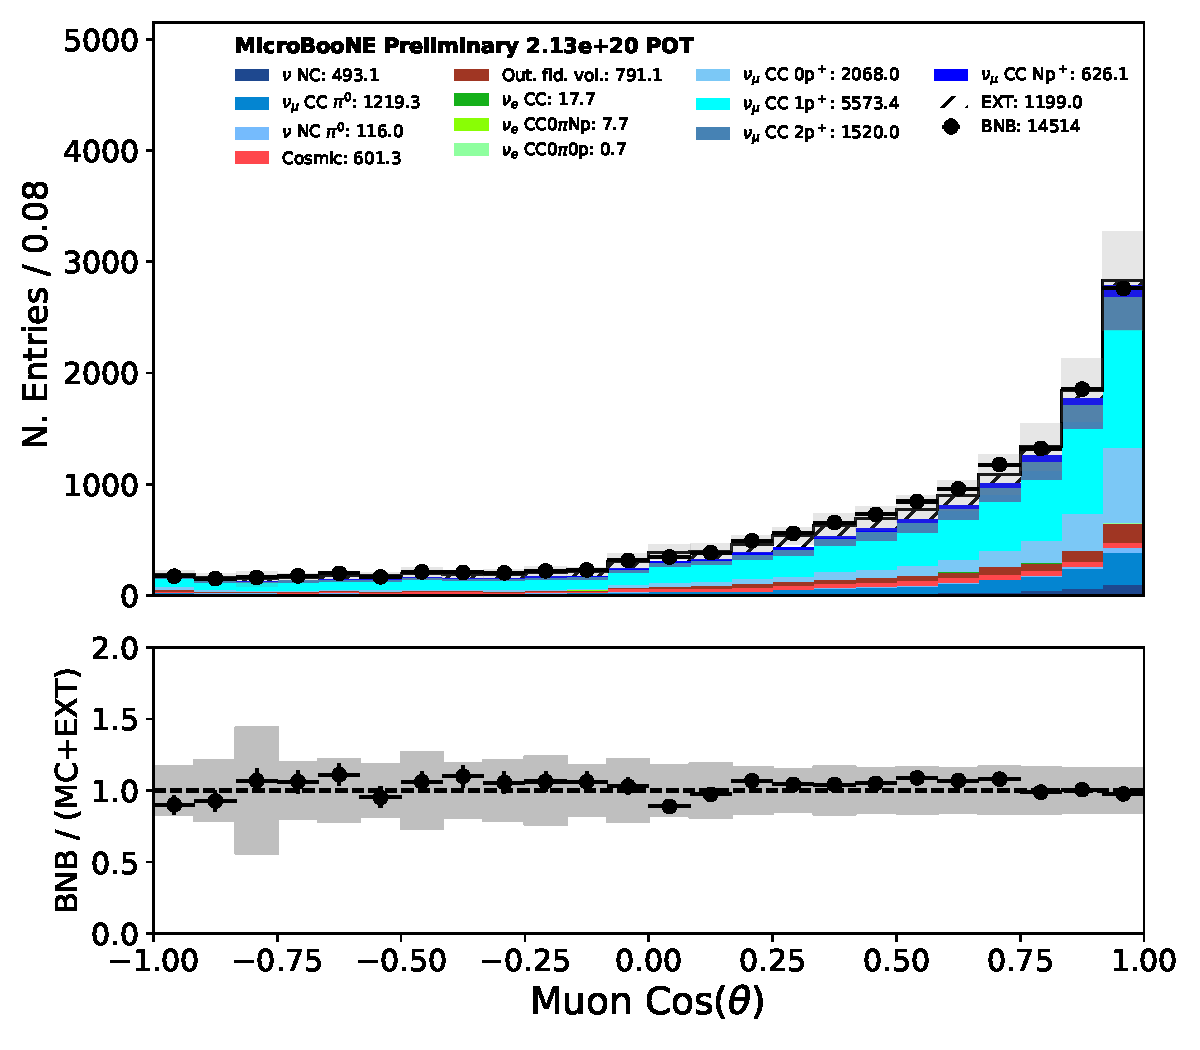
\includegraphics[width=1.00\textwidth]{NuMuCCsel/Images/Ryan/fullselection_run3_fullsystematics/trk_cos_theta_v_07232020_fullsel_samples_detsys_event_category.pdf}
        \caption{With CRT cuts.}
        \label{fig:NuMUCCsel:ryan:run3_costheta_withCRT}
    \end{subfigure}
    \begin{subfigure}[b]{0.35\textwidth}
        \centering
        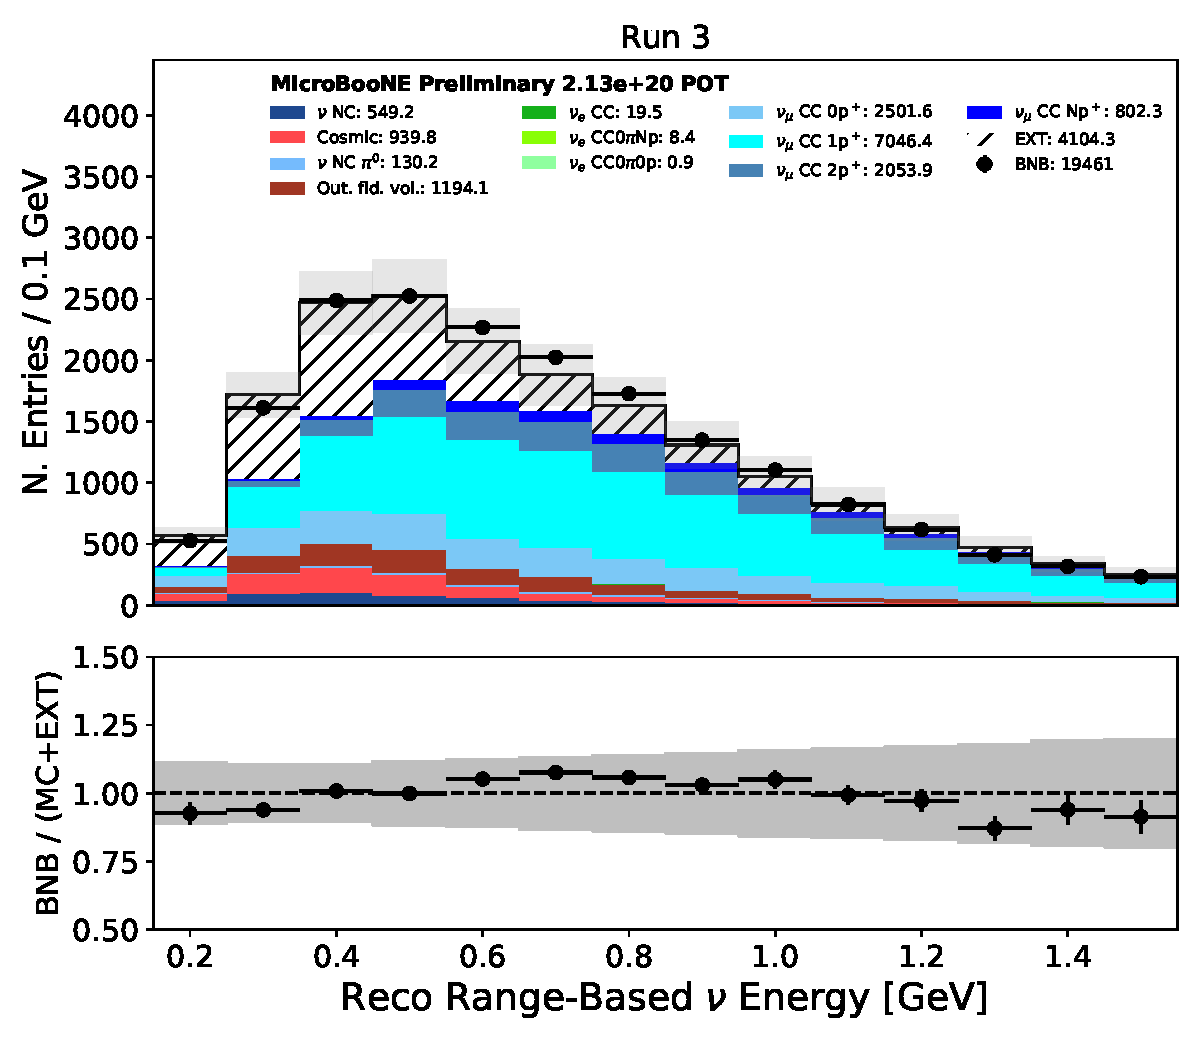
\includegraphics[width=1.00\textwidth]{NuMuCCsel/Images/Ryan/Run3_nocrt/reco_nu_e_range_v_08052020_full_samples_longest_noCRT_event_category.pdf}
        \caption{No CRT cuts.}
        \label{fig:NuMUCCsel:ryan:run3_Enu_noCRT}
    \end{subfigure}
    \begin{subfigure}[b]{0.35\textwidth}
        \centering
        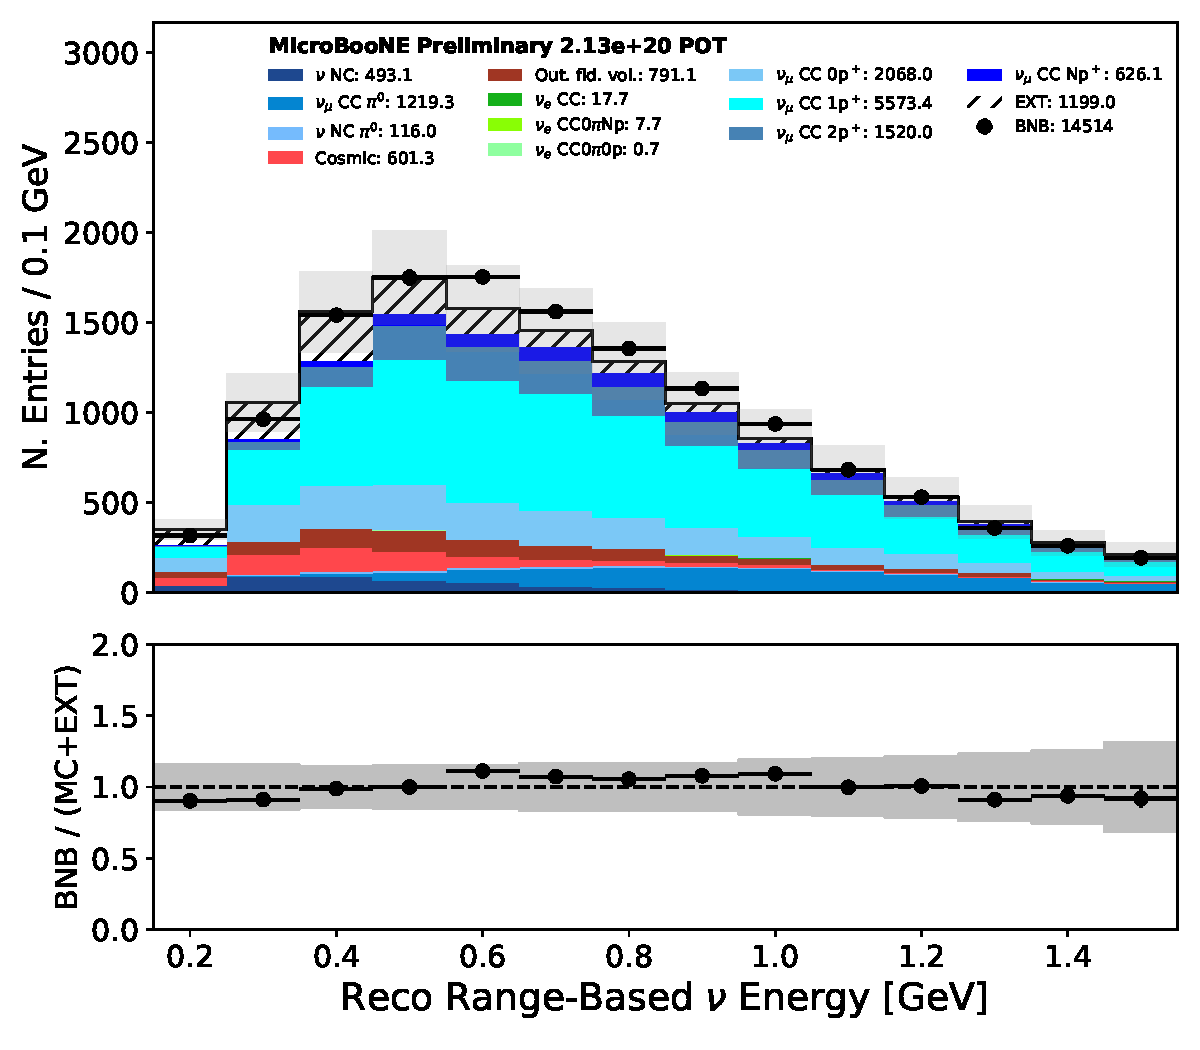
\includegraphics[width=1.00\textwidth]{NuMuCCsel/Images/Ryan/fullselection_run3_fullsystematics/reco_nu_e_range_v_07232020_fullsel_samples_detsys_event_category.pdf}
        \caption{With CRT cuts.}
        \label{fig:NuMUCCsel:ryan:run3_Enu_withCRT}
    \end{subfigure}
\caption{Impact of CRT cuts.}
\label{fig:NuMuCCsel:crtimpact}
\end{center}
\end{figure}

\subsection{Time Dependence}
\label{ssec:Appendix:numu:timedep}
%--------------------------- TIME DEPENDENCE STUDIES ----------------------
\begin{figure}[H] 
\begin{center}
    \begin{subfigure}[b]{0.35\textwidth}
        \centering
        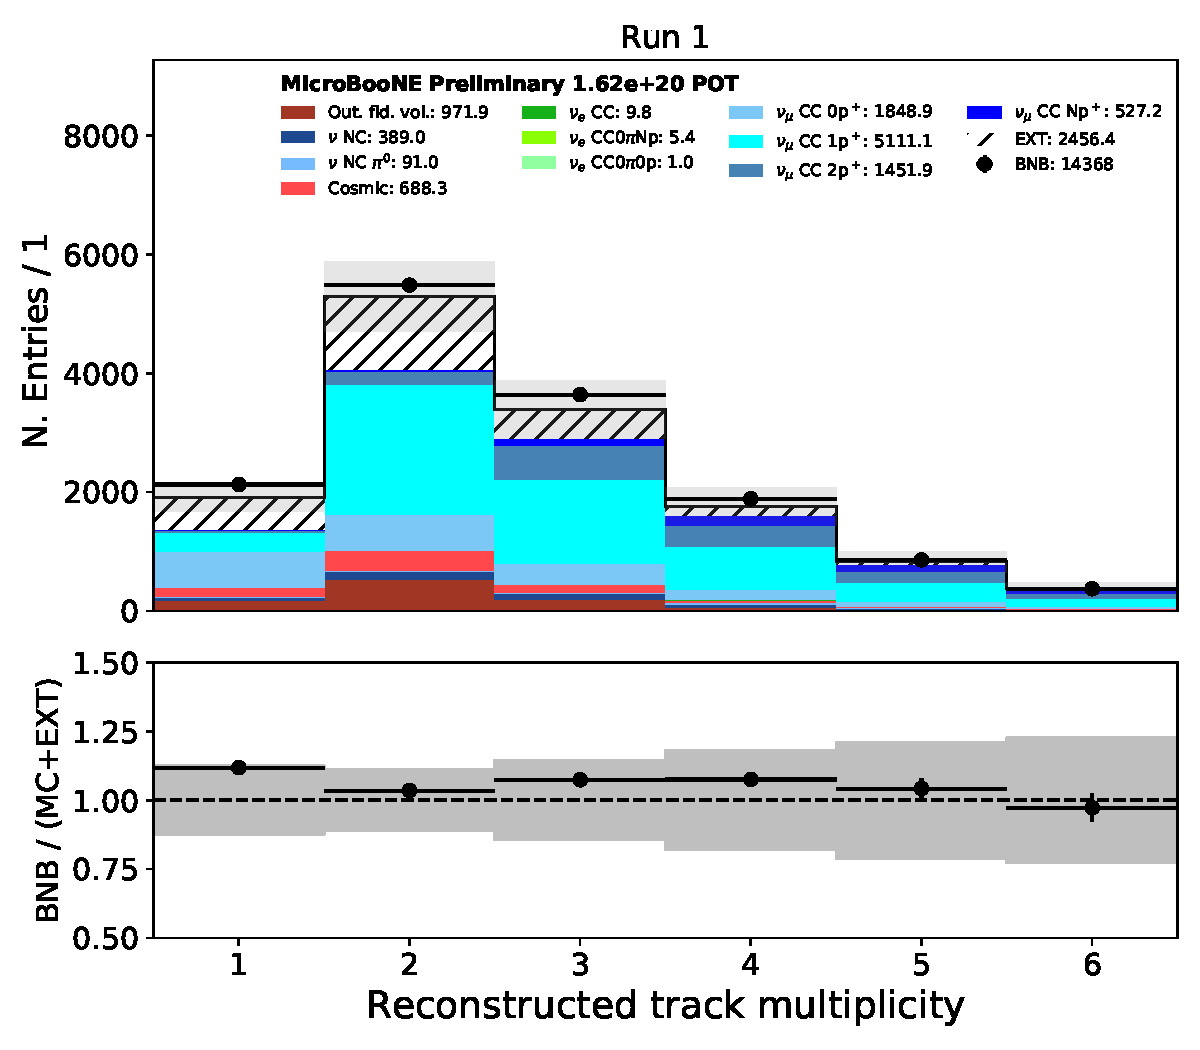
\includegraphics[width=1.00\textwidth]{NuMuCCsel/Images/Ryan/Run1/reco_ntrack_08052020_full_samples_longest_noCRT_event_category.pdf}
    \end{subfigure}
    \begin{subfigure}[b]{0.35\textwidth}
        \centering
        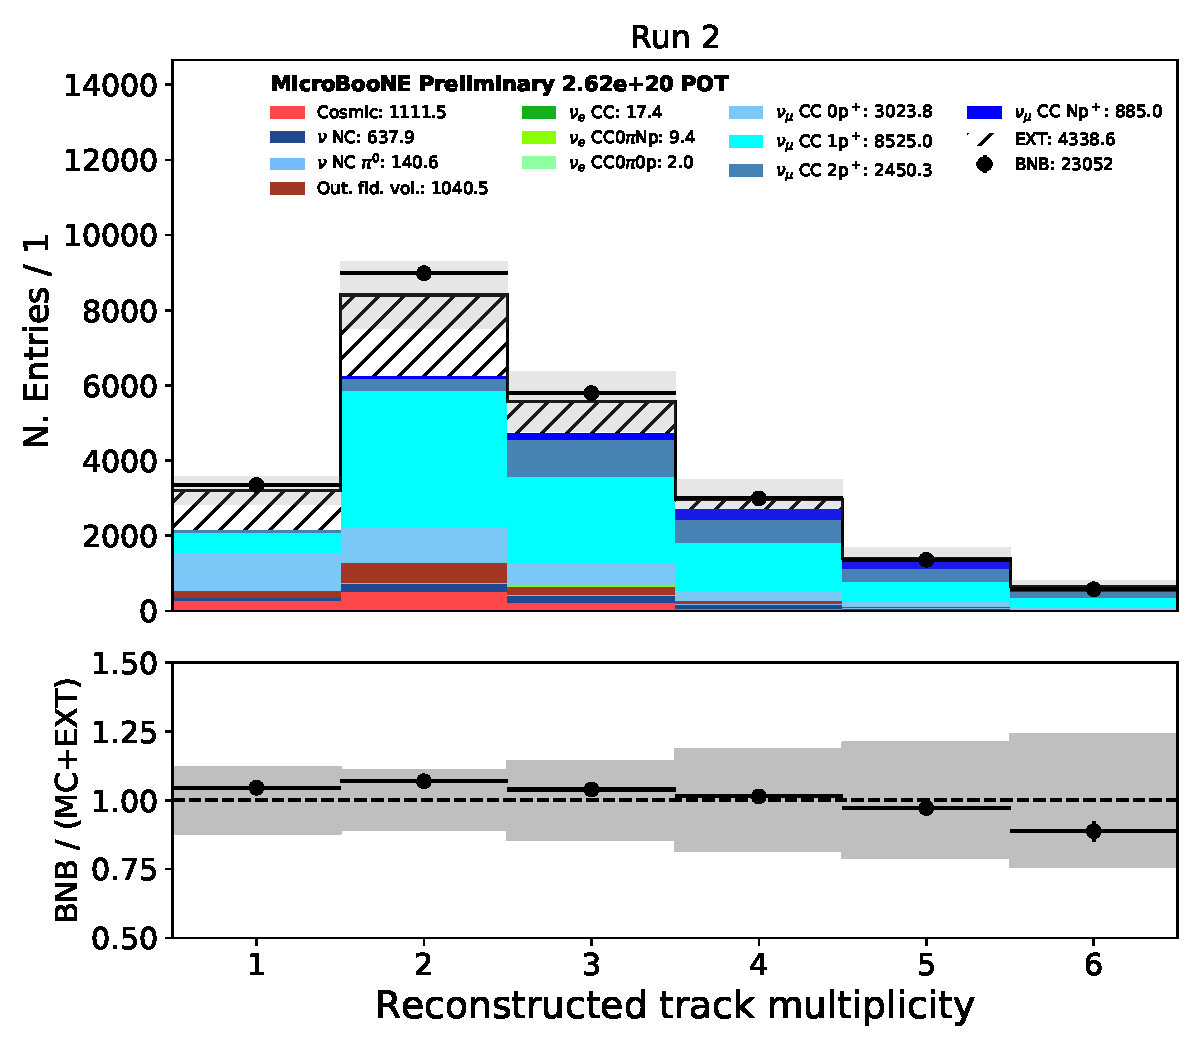
\includegraphics[width=1.00\textwidth]{NuMuCCsel/Images/Ryan/Run2/reco_ntrack_08052020_full_samples_longest_noCRT_event_category.pdf}
    \end{subfigure}
    \begin{subfigure}[b]{0.35\textwidth}
        \centering
        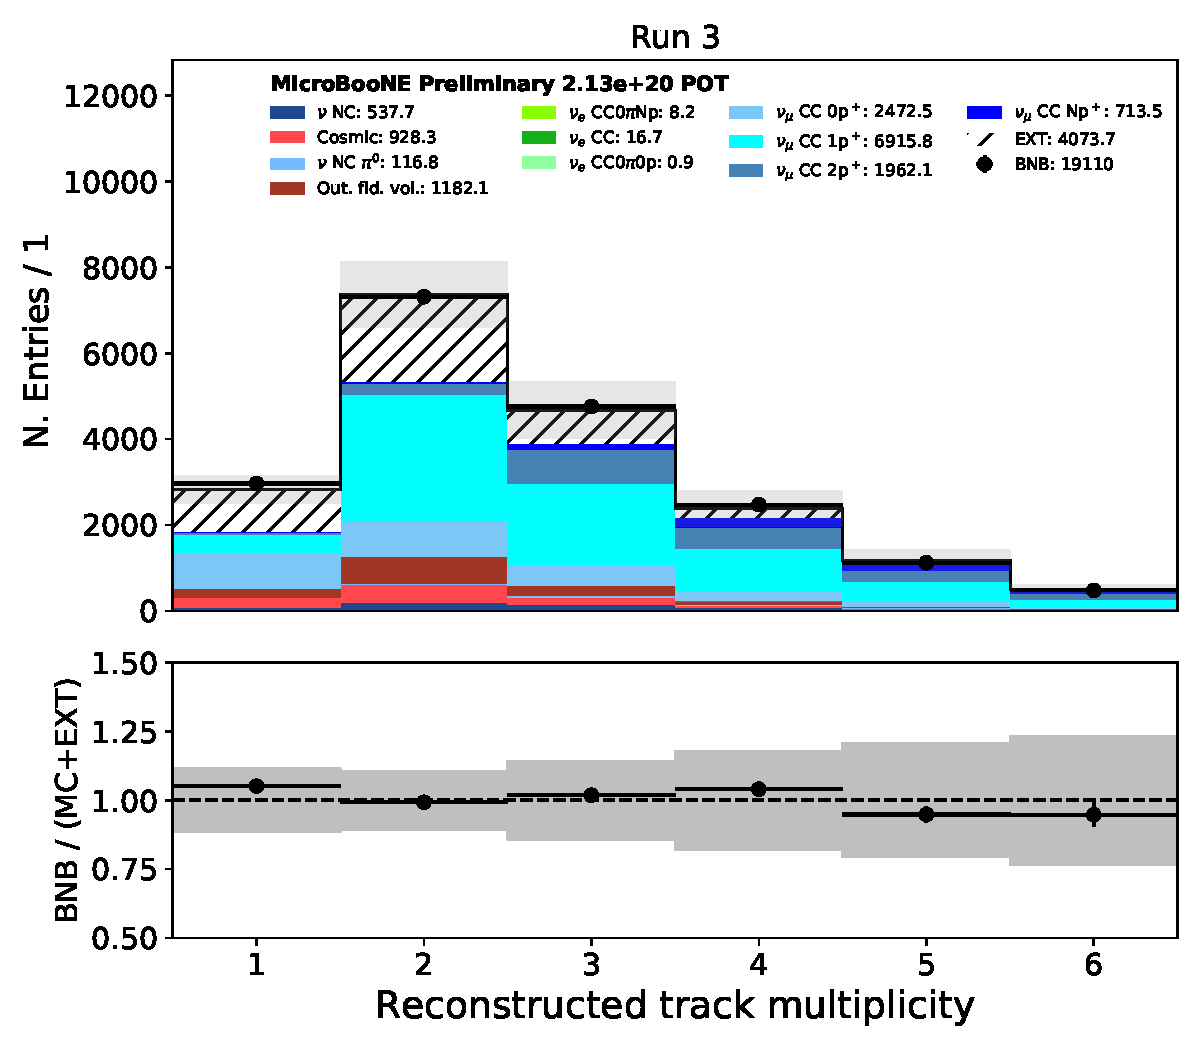
\includegraphics[width=1.00\textwidth]{NuMuCCsel/Images/Ryan/Run3_nocrt/reco_ntrack_08052020_full_samples_longest_noCRT_event_category.pdf}
    \end{subfigure} %\newline
    \begin{subfigure}[b]{0.35\textwidth}
        \centering
        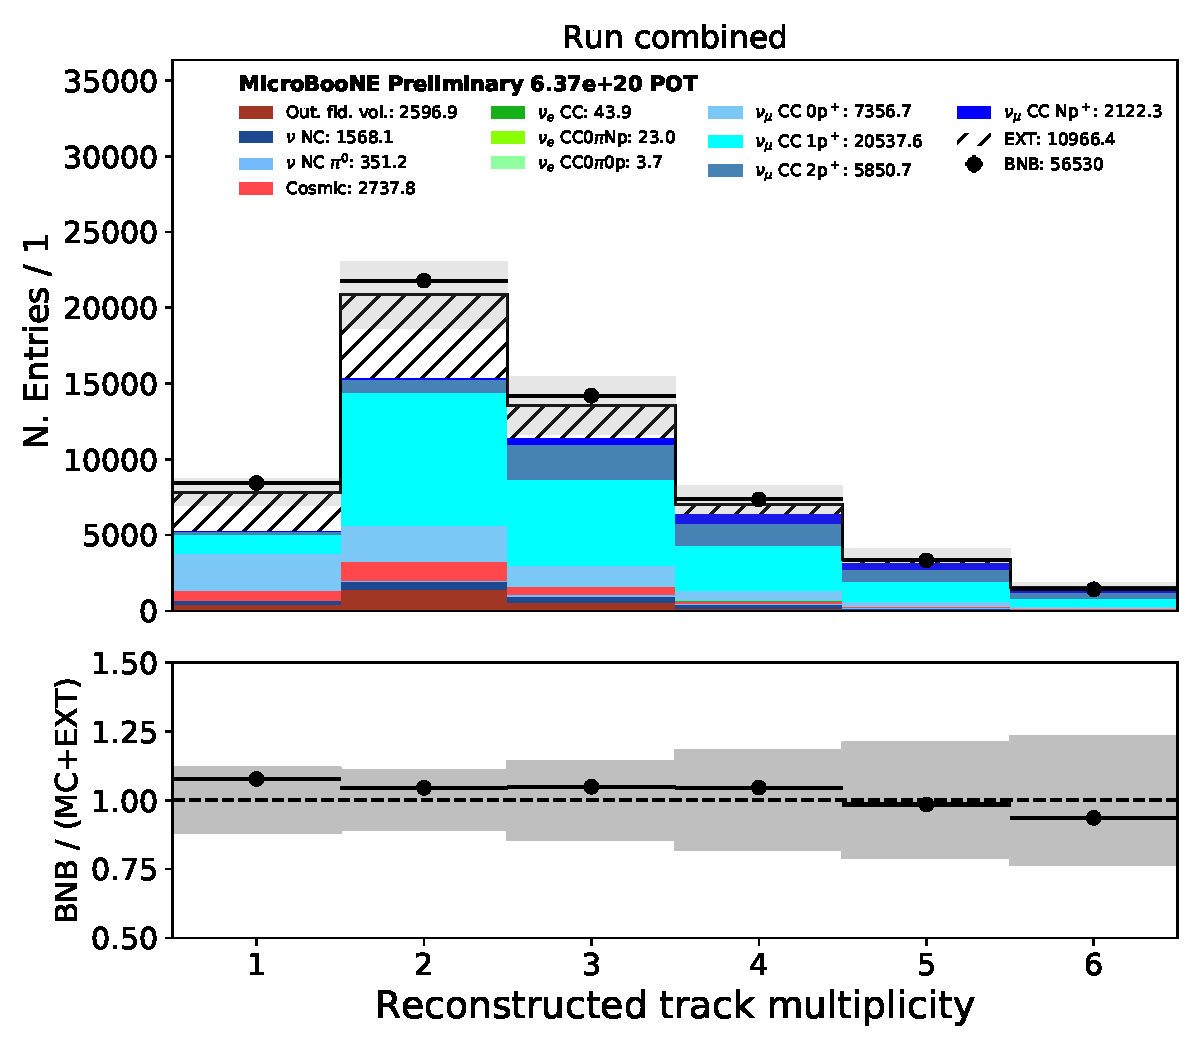
\includegraphics[width=1.00\textwidth]{NuMuCCsel/Images/Ryan/combined/reco_ntrack_08052020_full_samples_longest_noCRT_event_category.pdf}
    \end{subfigure}
\caption{Time dependence of track multiplicity for full $\nu_{\mu}$ CC INC selection.}
\label{fig:NuMuCCsel:timedep:ntrack}
\end{center}
\end{figure}

\begin{figure}[H] 
\begin{center}
    \begin{subfigure}[b]{0.35\textwidth}
        \centering
        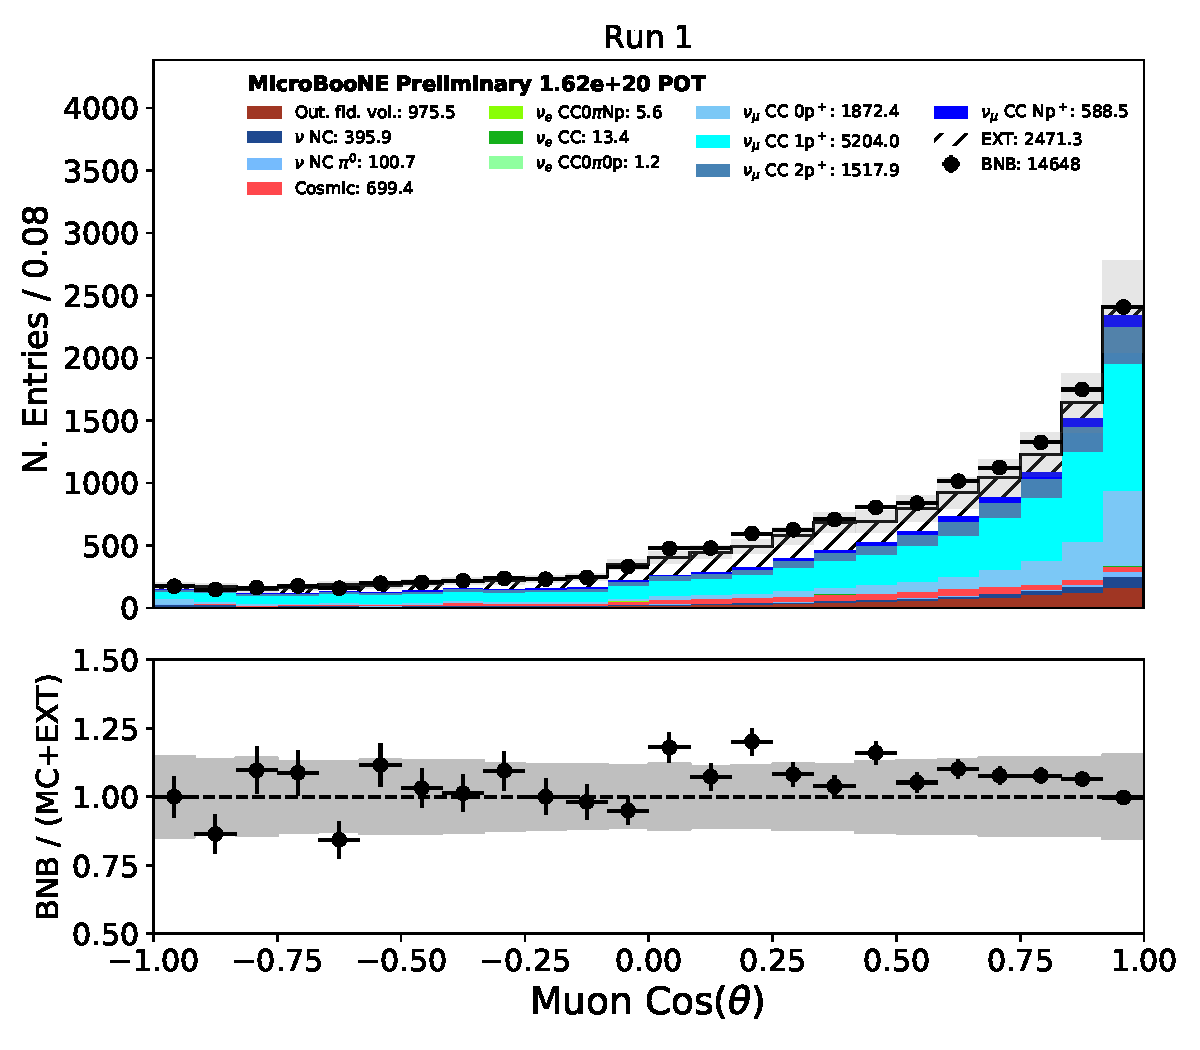
\includegraphics[width=1.00\textwidth]{NuMuCCsel/Images/Ryan/Run1/trk_cos_theta_v_08052020_full_samples_longest_noCRT_event_category.pdf}
    \end{subfigure}
    \begin{subfigure}[b]{0.35\textwidth}
        \centering
        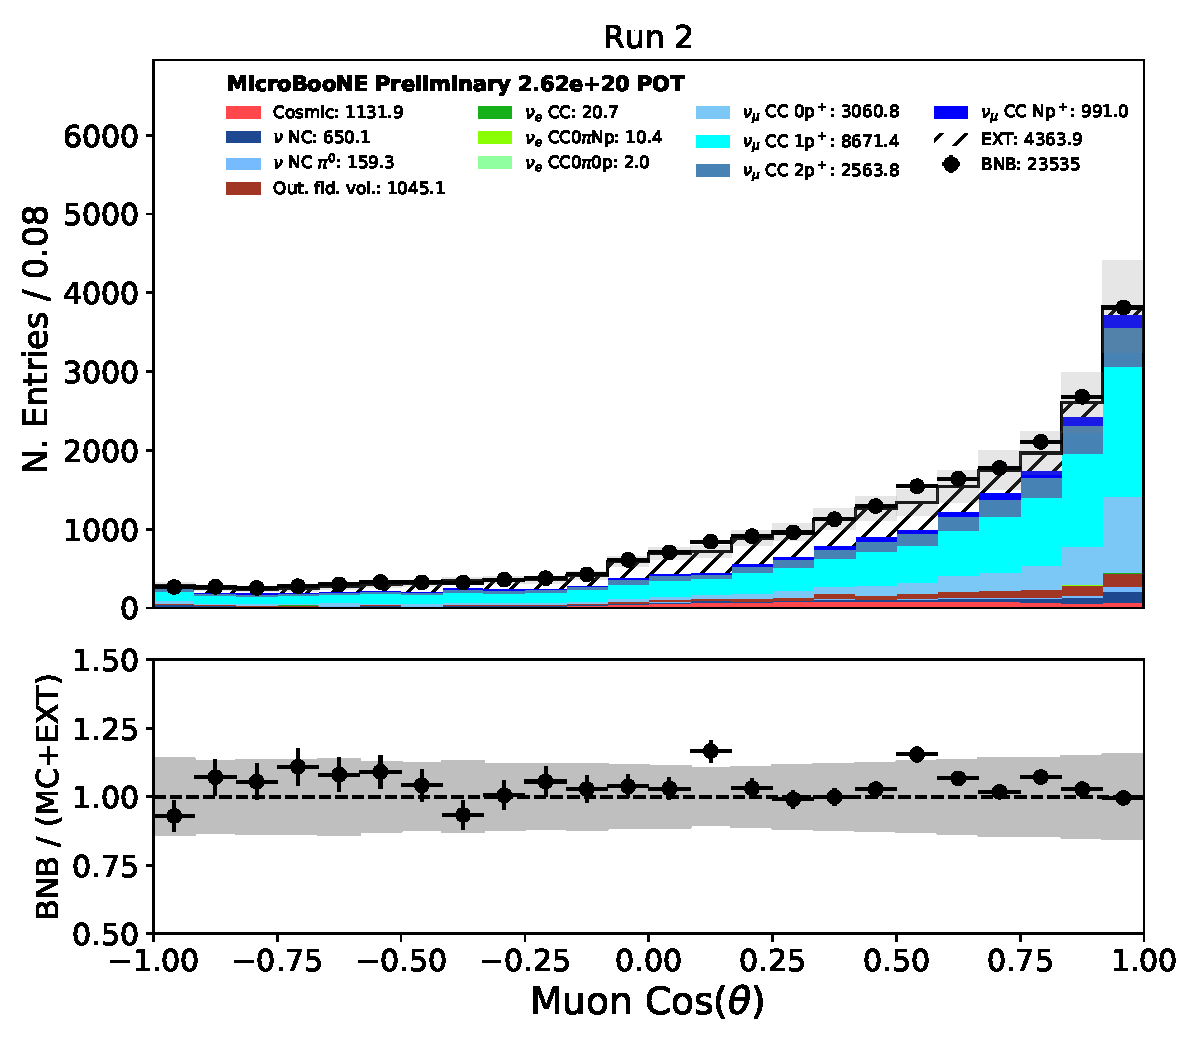
\includegraphics[width=1.00\textwidth]{NuMuCCsel/Images/Ryan/Run2/trk_cos_theta_v_08052020_full_samples_longest_noCRT_event_category.pdf}
    \end{subfigure}
    \begin{subfigure}[b]{0.35\textwidth}
        \centering
        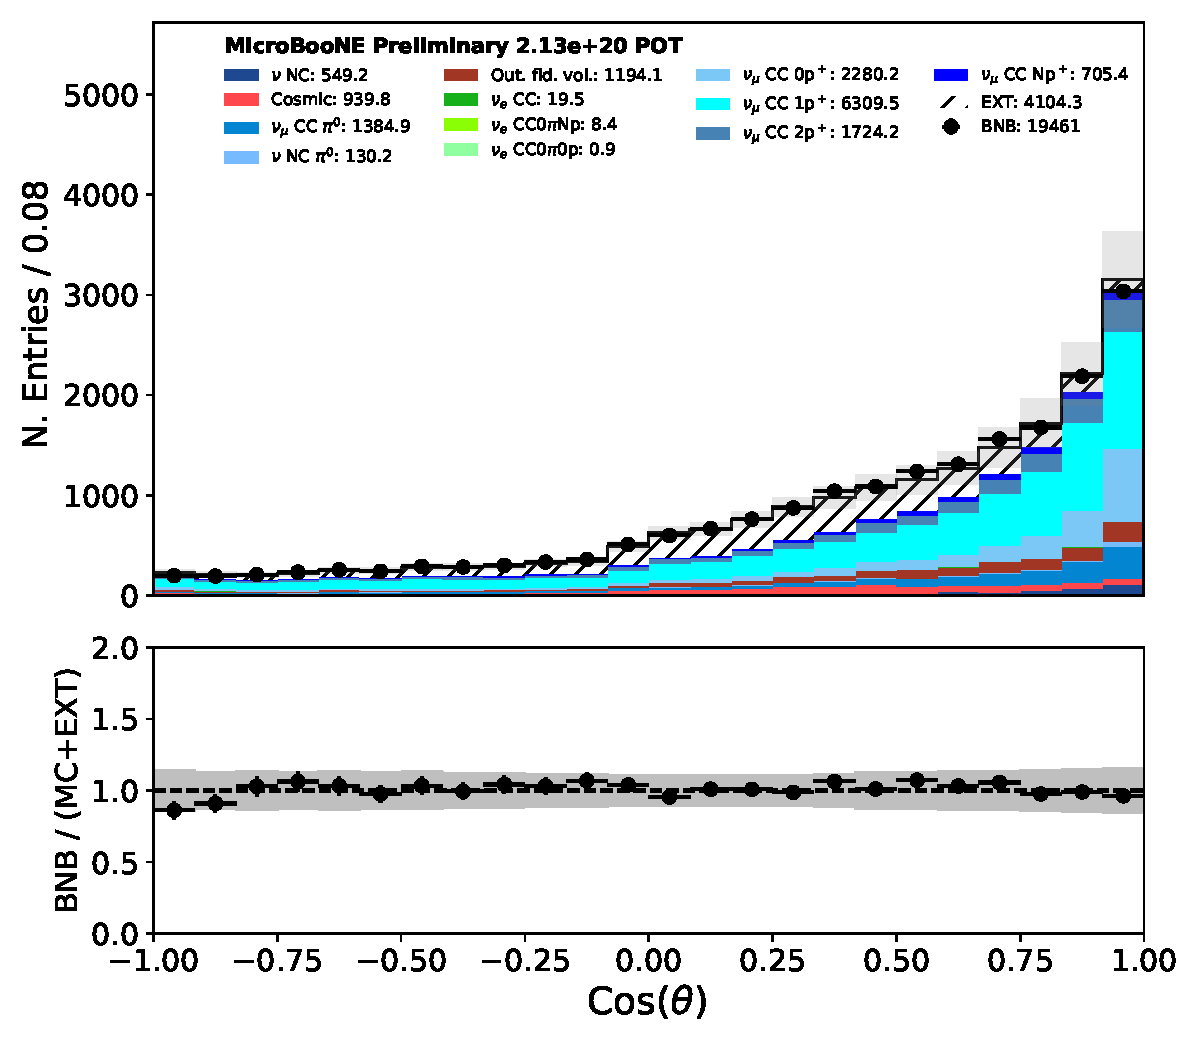
\includegraphics[width=1.00\textwidth]{NuMuCCsel/Images/Ryan/Run3_nocrt/trk_cos_theta_08052020_fullsel_samples_event_category_noCRT.pdf}
    \end{subfigure} %\newline
    \begin{subfigure}[b]{0.35\textwidth}
        \centering
        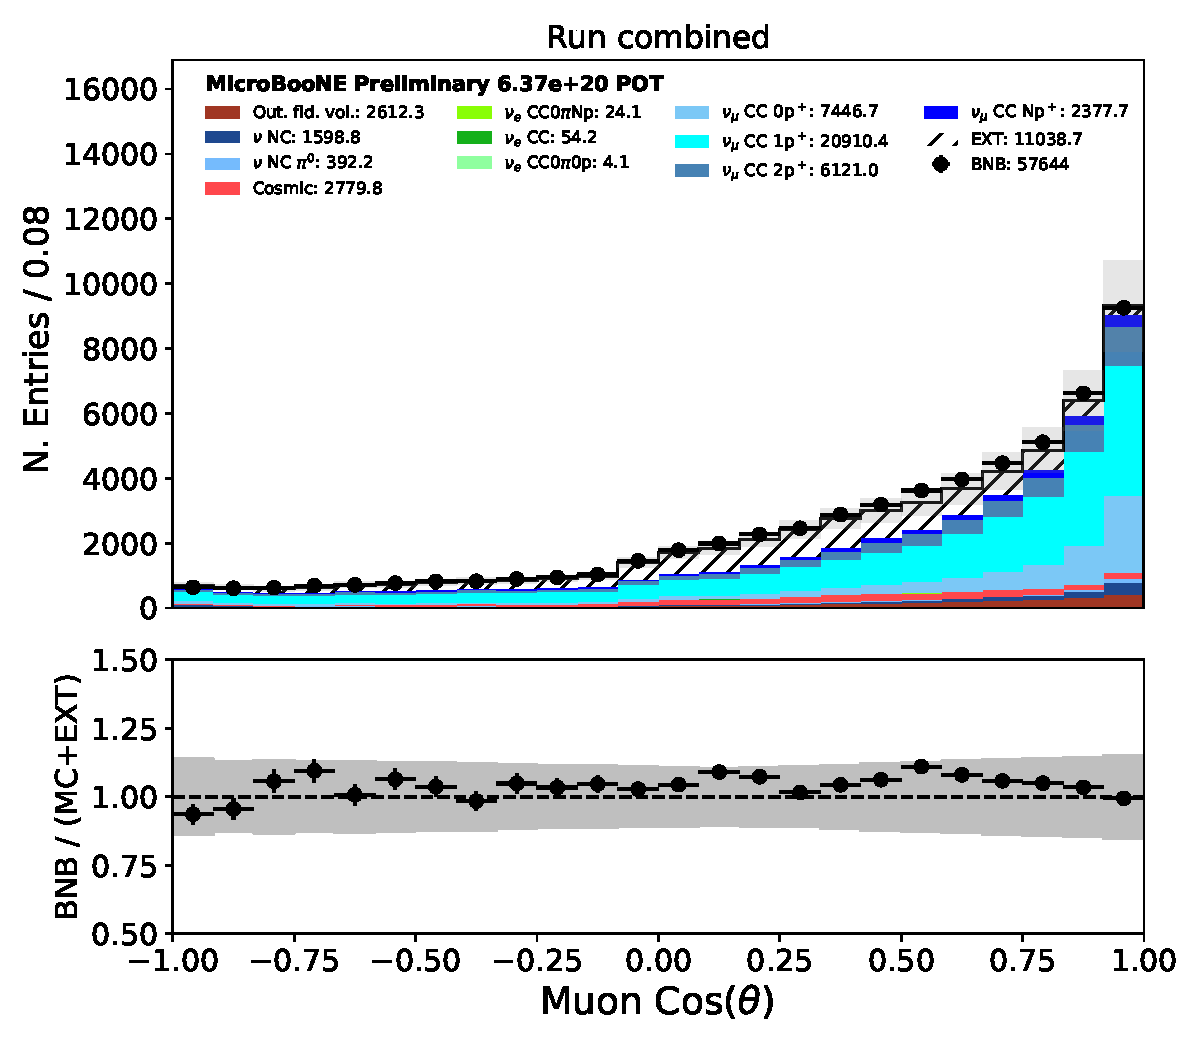
\includegraphics[width=1.00\textwidth]{NuMuCCsel/Images/Ryan/combined/trk_cos_theta_v_08052020_full_samples_longest_noCRT_event_category.pdf}
    \end{subfigure}
\caption{Time dependence of reconstructed muon angle about beam axis for full $\nu_{\mu}$ CC INC selection.}
\label{fig:NuMuCCsel:timedep:costheta}
\end{center}
\end{figure}

\begin{figure}[hbt!] 
\begin{center}
    \begin{subfigure}[b]{0.35\textwidth}
        \centering
        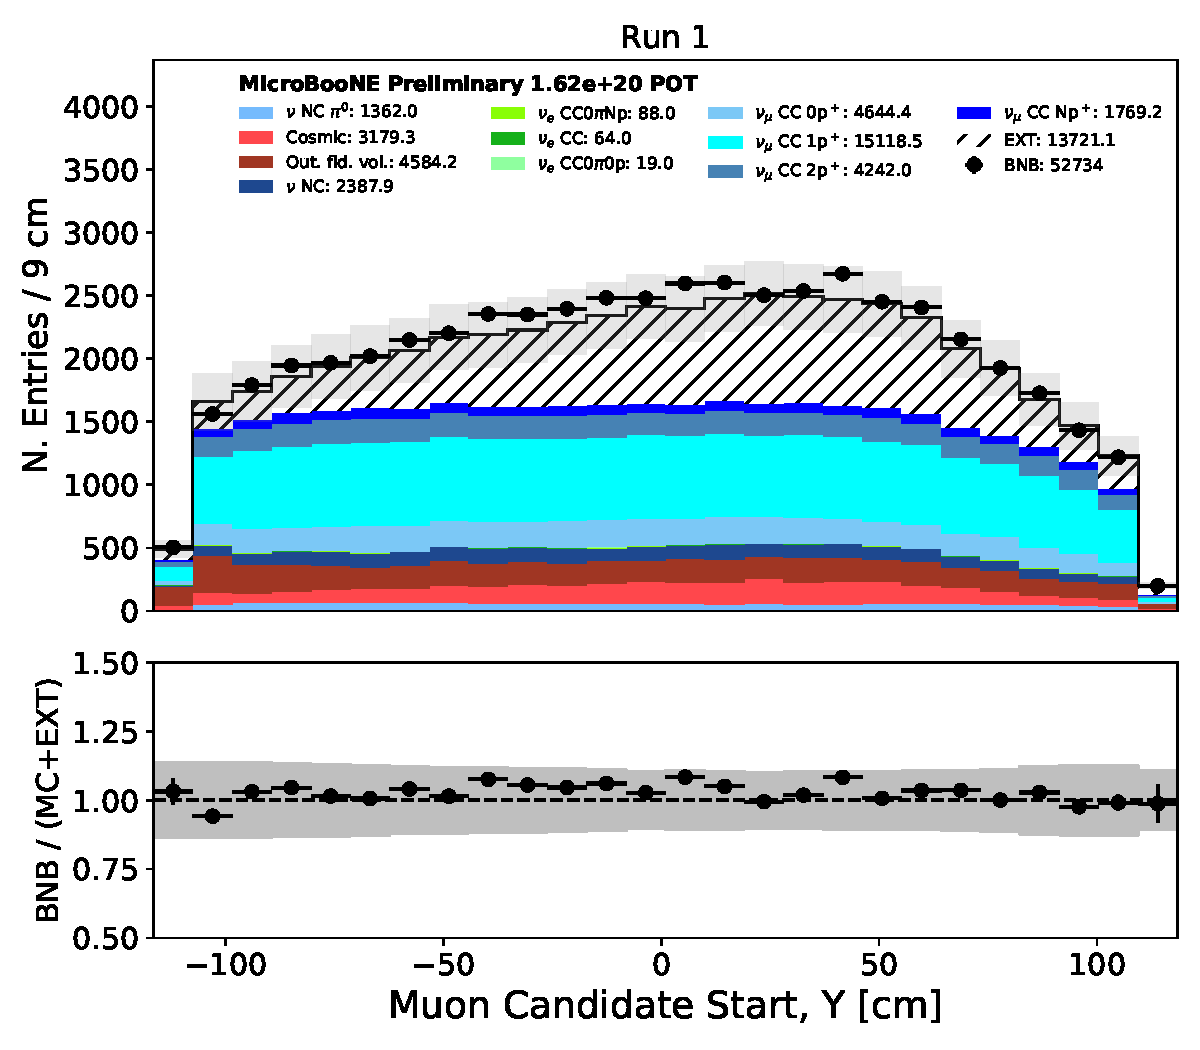
\includegraphics[width=1.00\textwidth]{NuMuCCsel/Images/Ryan/Run1/trk_sce_start_y_v_08052020_presel_samples_longest_noCRT_event_category.pdf}
    \end{subfigure}
    \begin{subfigure}[b]{0.35\textwidth}
        \centering
        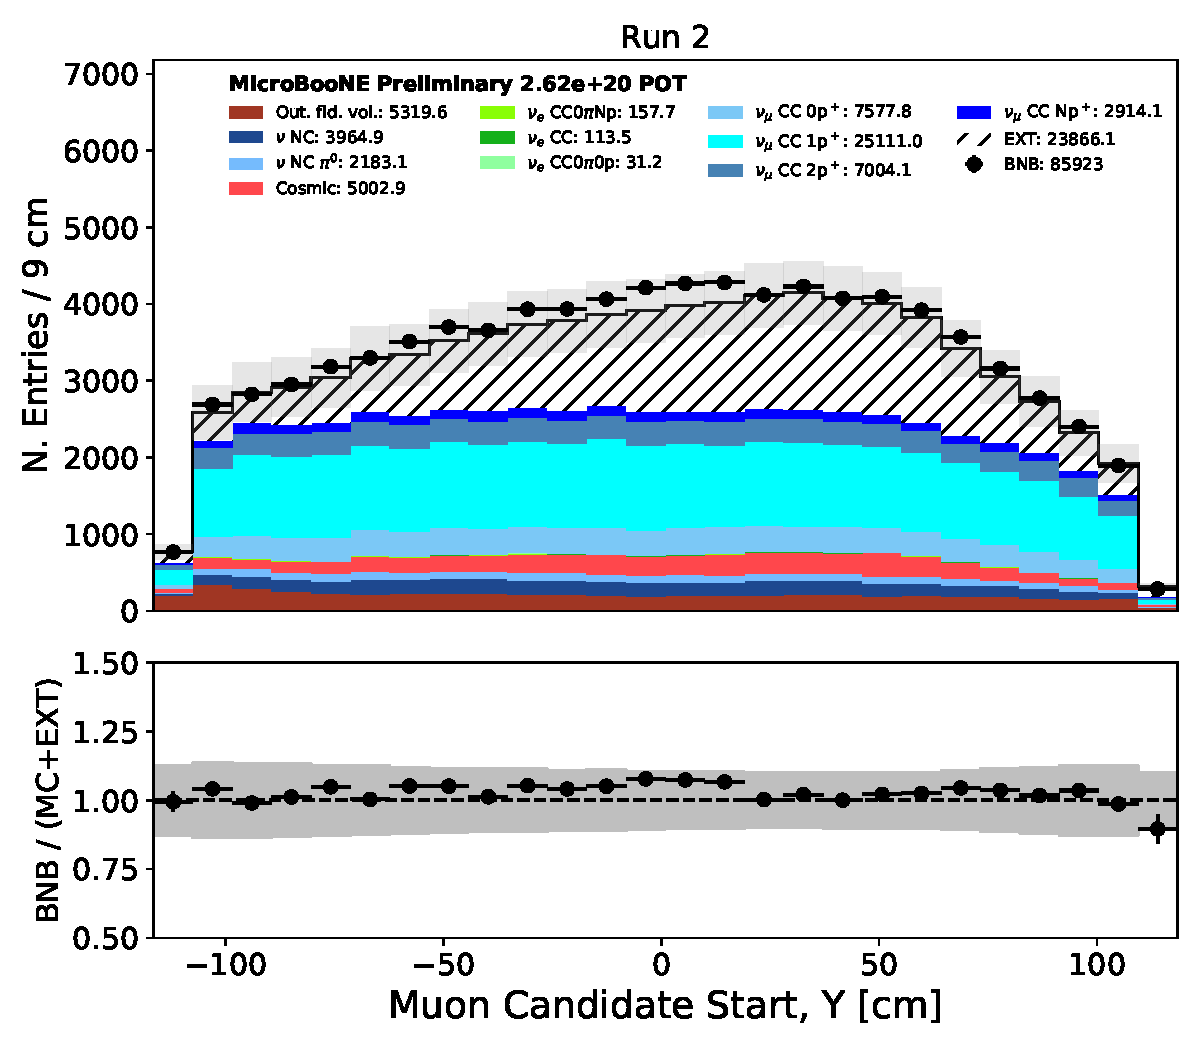
\includegraphics[width=1.00\textwidth]{NuMuCCsel/Images/Ryan/Run2/trk_sce_start_y_v_08052020_presel_samples_longest_noCRT_event_category.pdf}
    \end{subfigure}
    \begin{subfigure}[b]{0.35\textwidth}
        \centering
        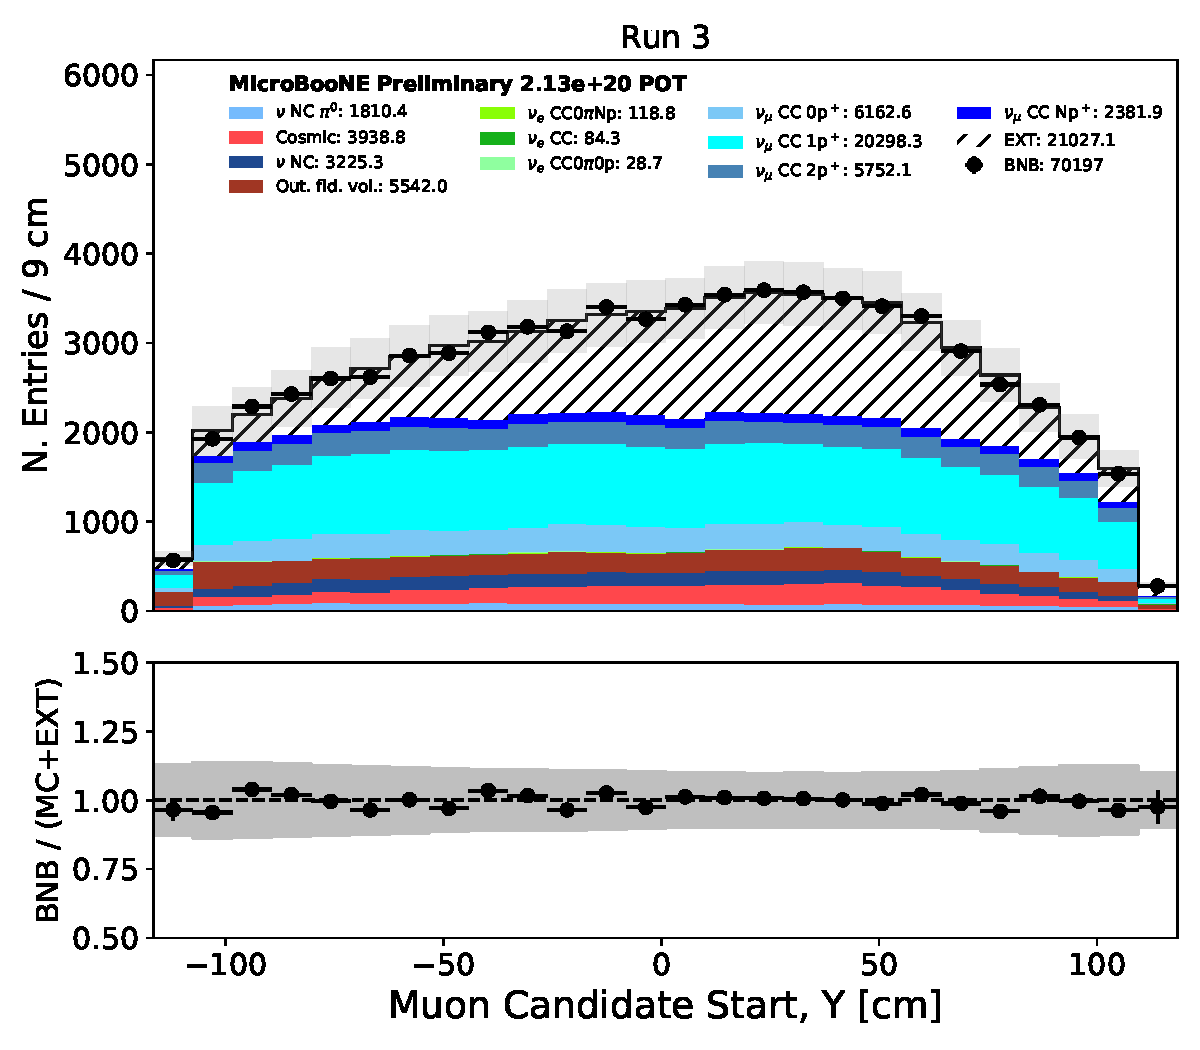
\includegraphics[width=1.00\textwidth]{NuMuCCsel/Images/Ryan/Run3_nocrt/trk_sce_start_y_v_08052020_presel_samples_longest_noCRT_event_category.pdf}
    \end{subfigure} %\newline
    \begin{subfigure}[b]{0.35\textwidth}
        \centering
        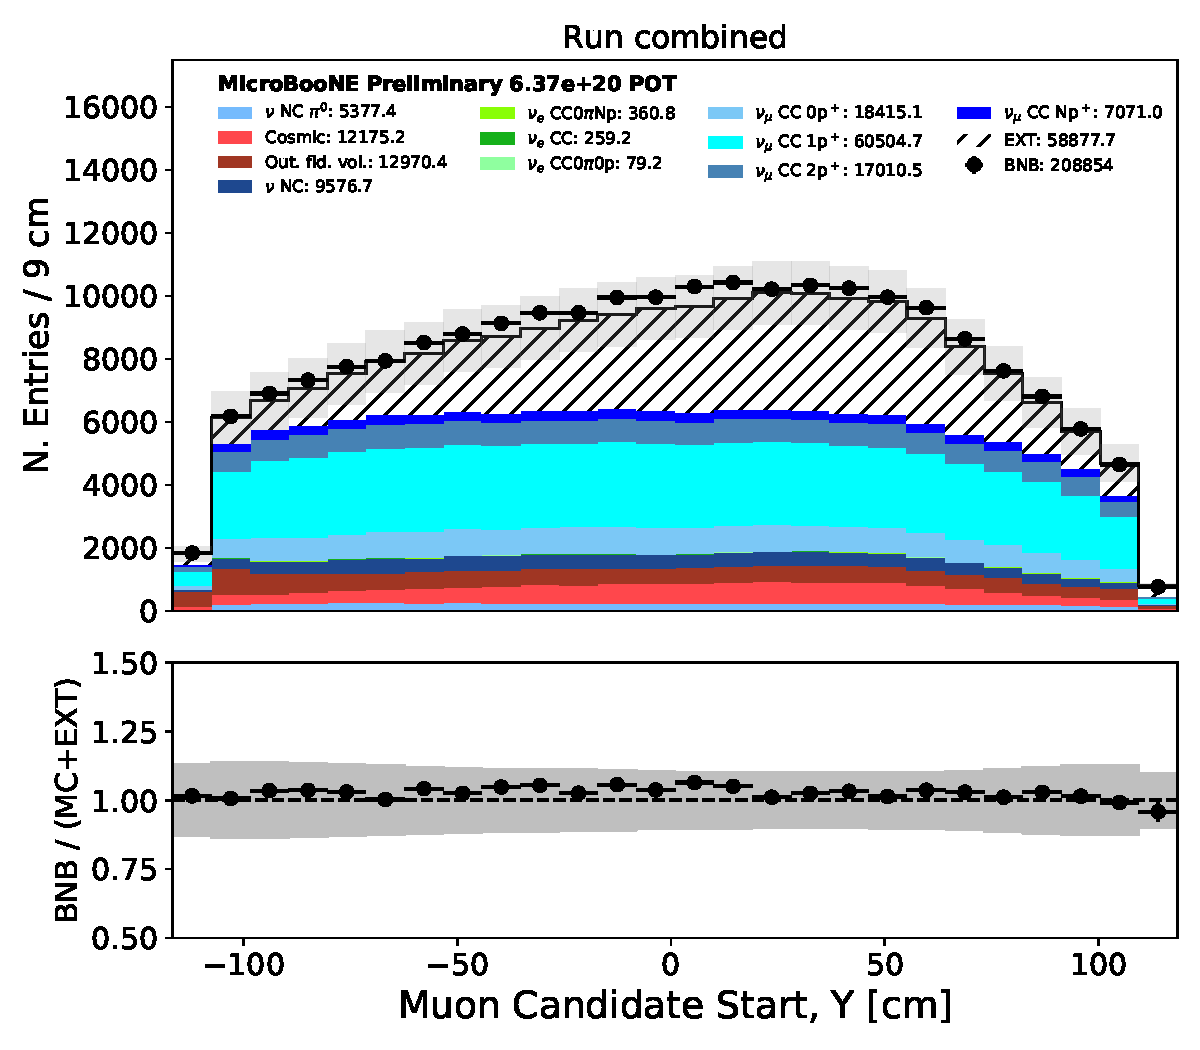
\includegraphics[width=1.00\textwidth]{NuMuCCsel/Images/Ryan/combined/trk_sce_start_y_v_08052020_presel_samples_longest_noCRT_event_category.pdf}
    \end{subfigure}
\caption{Time dependence of reconstructed Y coordinate of muon start points after preselection.}
\label{fig:NuMuCCsel:timedep:trkstarty}
\end{center}
\end{figure}

\begin{figure}[hbt!] 
\begin{center}
    \begin{subfigure}[b]{0.35\textwidth}
        \centering
        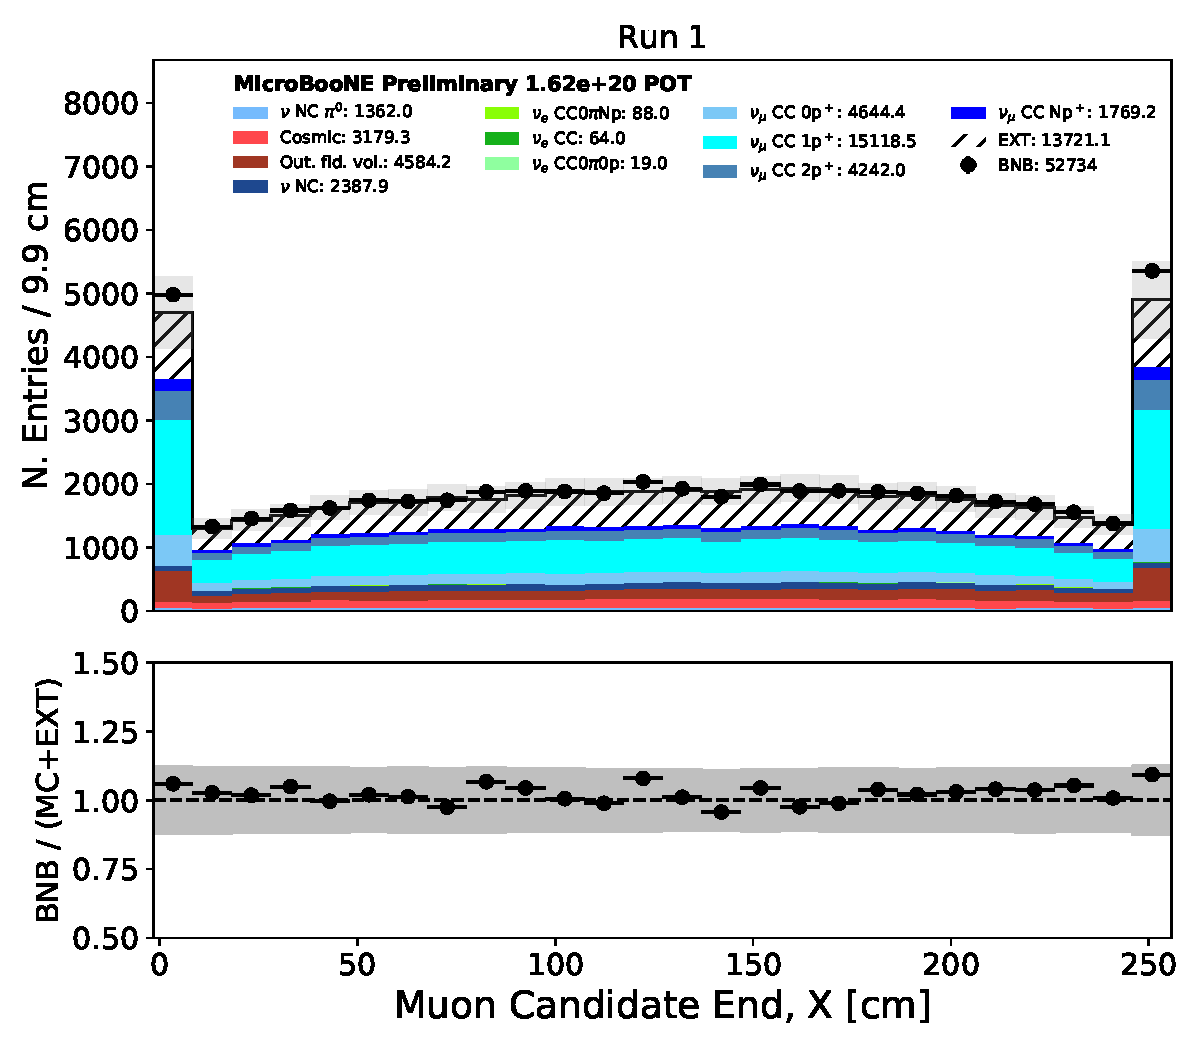
\includegraphics[width=1.00\textwidth]{NuMuCCsel/Images/Ryan/Run1/trk_sce_end_x_v_08052020_presel_samples_longest_noCRT_event_category.pdf}
    \end{subfigure}
    \begin{subfigure}[b]{0.35\textwidth}
        \centering
        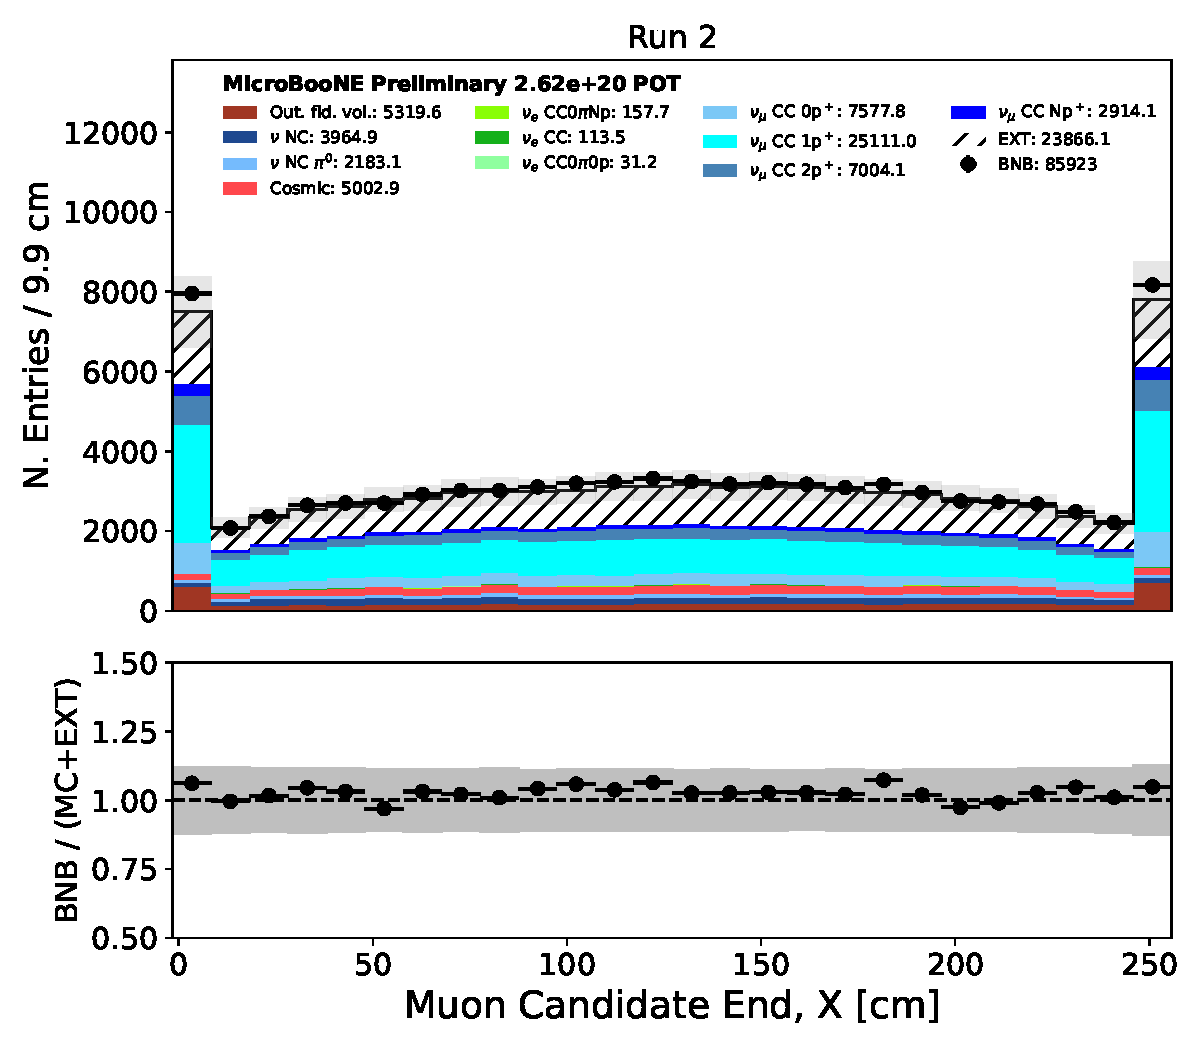
\includegraphics[width=1.00\textwidth]{NuMuCCsel/Images/Ryan/Run2/trk_sce_end_x_v_08052020_presel_samples_longest_noCRT_event_category.pdf}
    \end{subfigure}
    \begin{subfigure}[b]{0.35\textwidth}
        \centering
        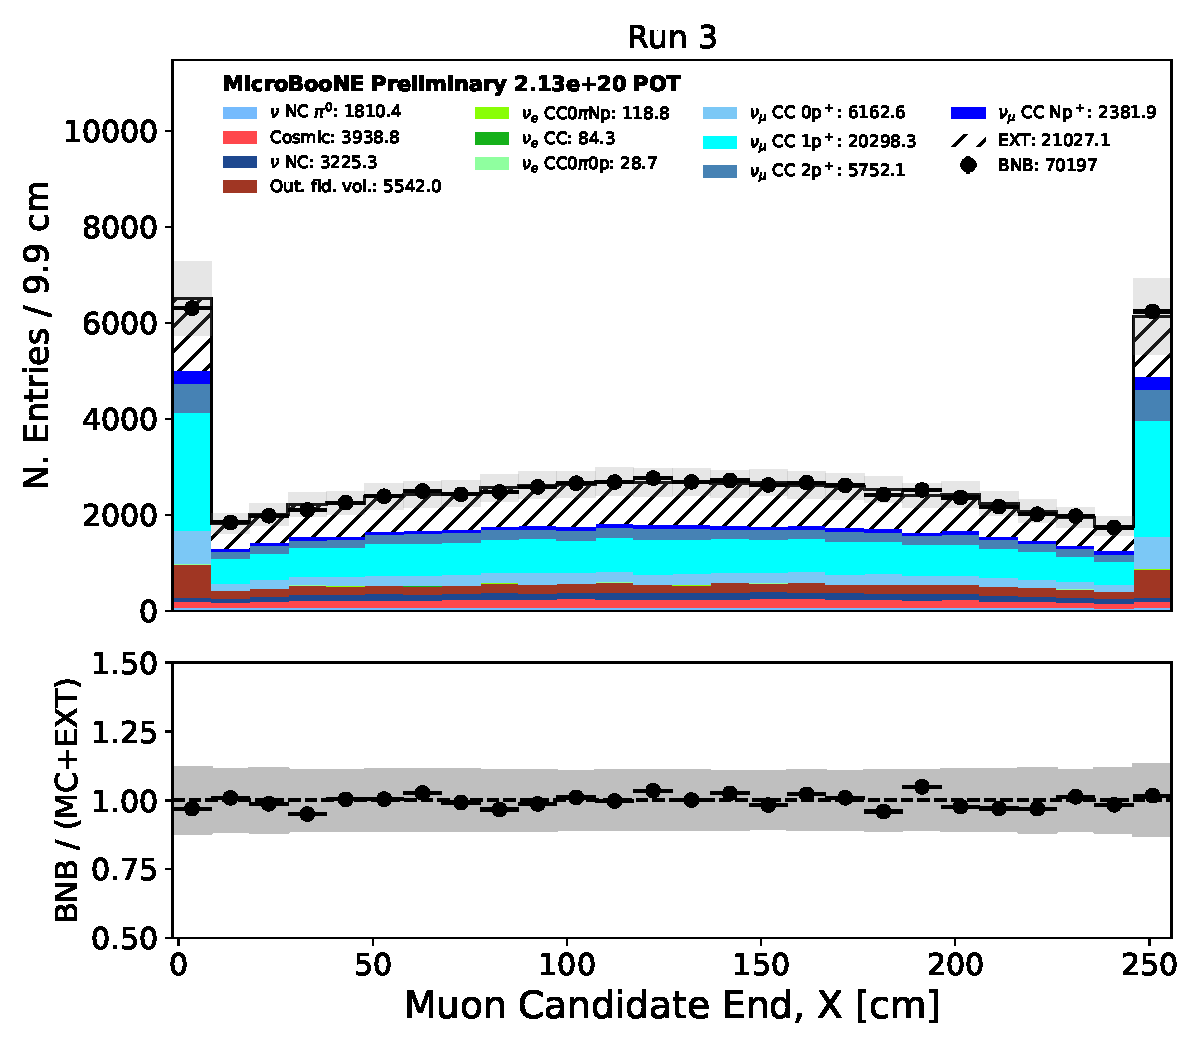
\includegraphics[width=1.00\textwidth]{NuMuCCsel/Images/Ryan/Run3_nocrt/trk_sce_end_x_v_08052020_presel_samples_longest_noCRT_event_category.pdf}
    \end{subfigure} %\newline
    \begin{subfigure}[b]{0.35\textwidth}
        \centering
        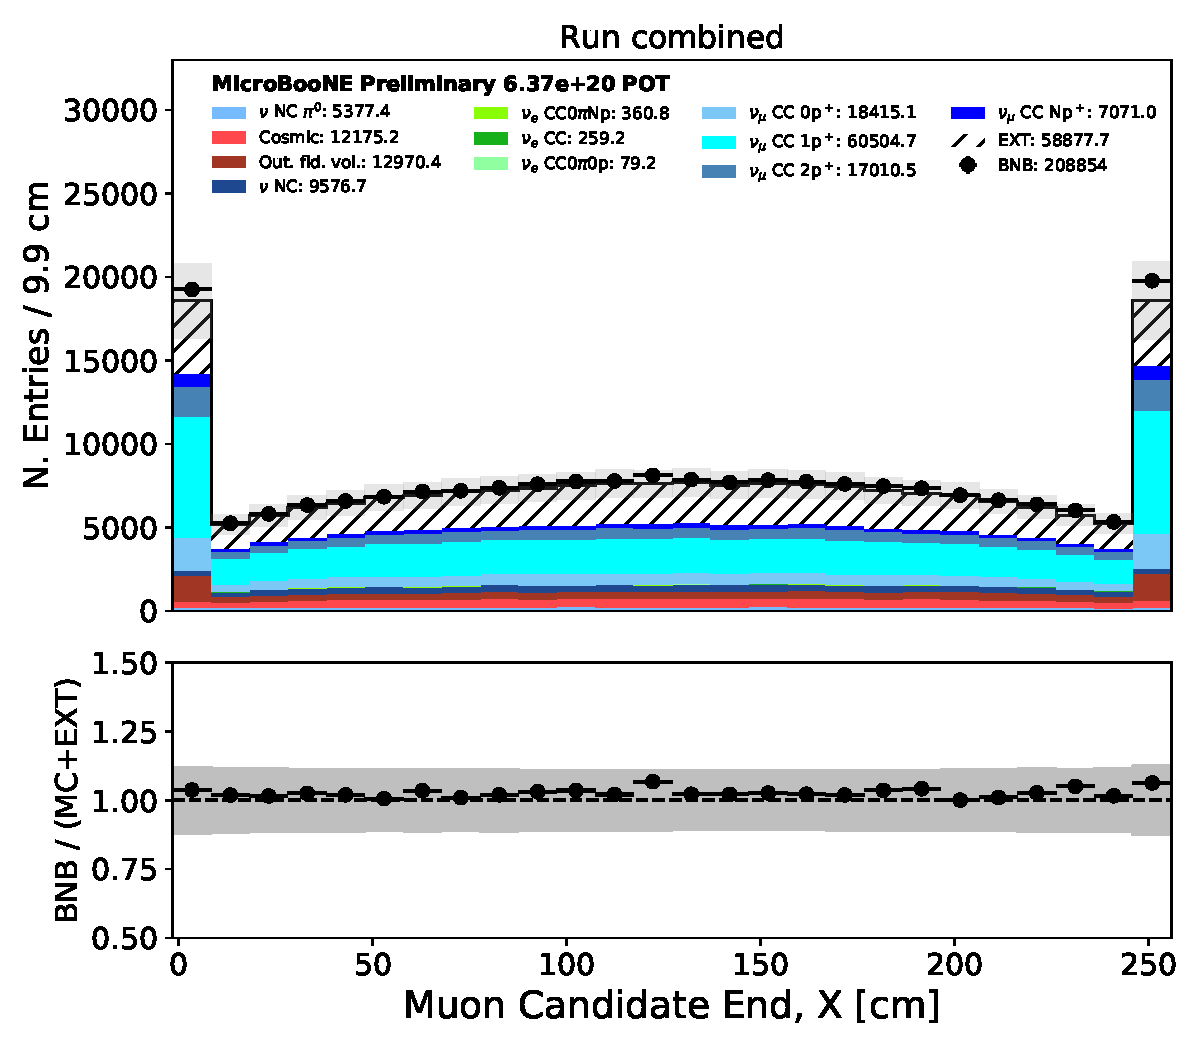
\includegraphics[width=1.00\textwidth]{NuMuCCsel/Images/Ryan/combined/trk_sce_end_x_v_08052020_presel_samples_longest_noCRT_event_category.pdf}
    \end{subfigure}
\caption{Time dependence of reconstructed X coordinate of muon end points after preselection.}
\label{fig:NuMuCCsel:timedep:trkendx}
\end{center}
\end{figure}

\begin{figure}[hbt!] 
\begin{center}
    \begin{subfigure}[b]{0.35\textwidth}
        \centering
        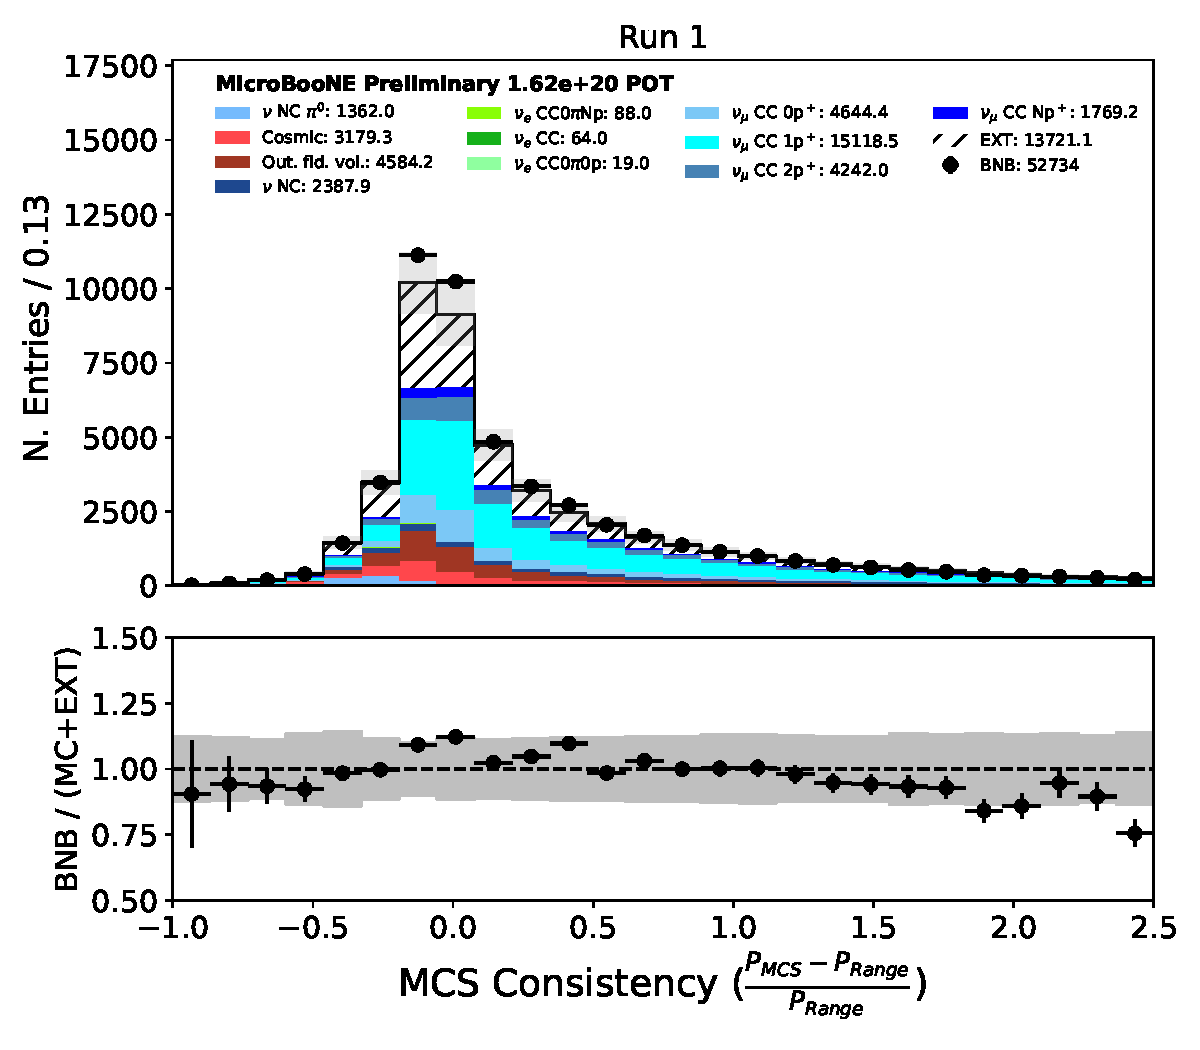
\includegraphics[width=1.00\textwidth]{NuMuCCsel/Images/Ryan/Run1/trk_p_quality_v_08052020_presel_samples_longest_noCRT_event_category.pdf}
    \end{subfigure}
    \begin{subfigure}[b]{0.35\textwidth}
        \centering
        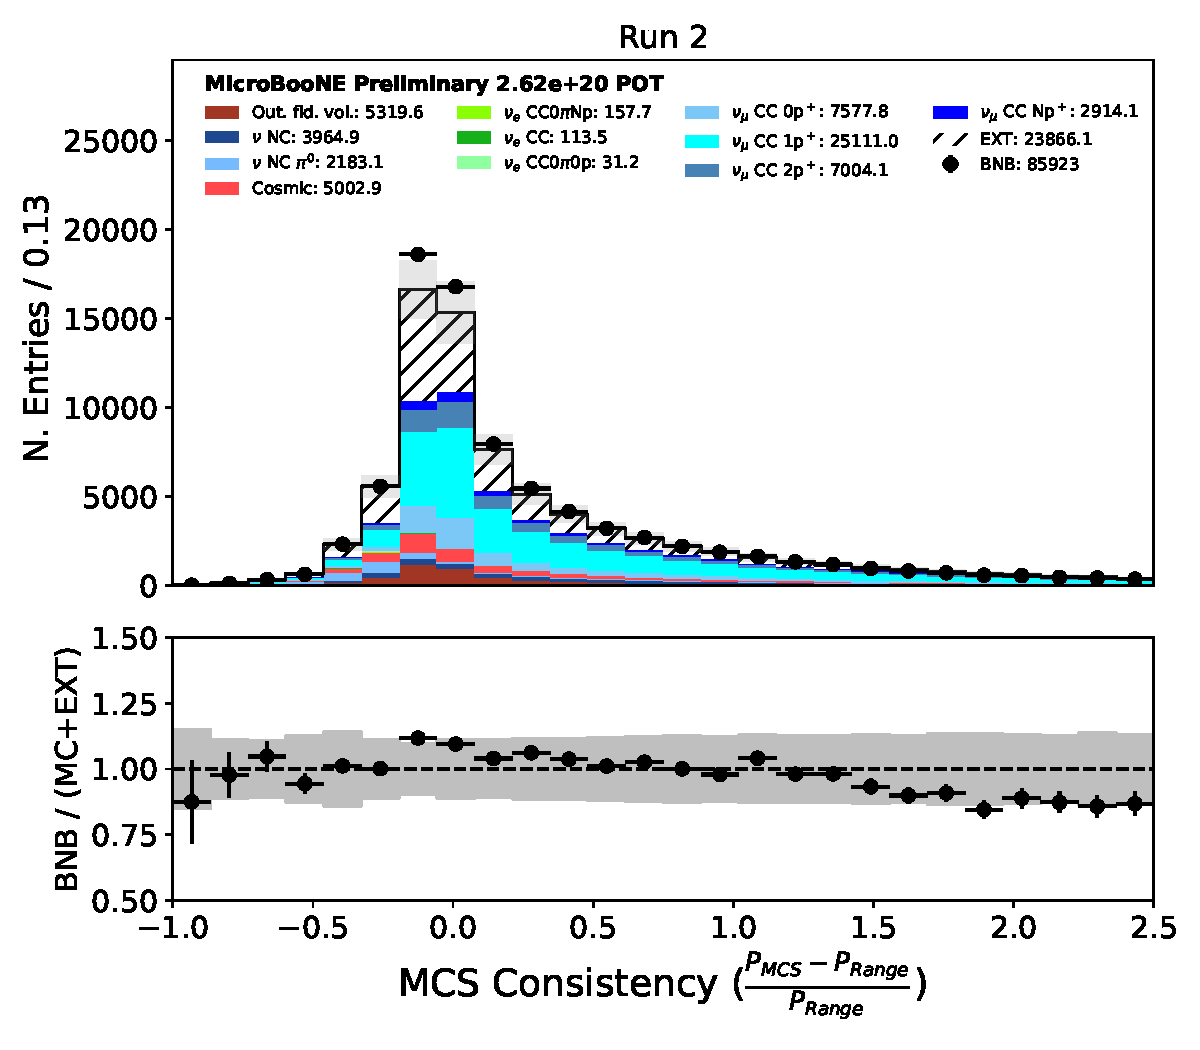
\includegraphics[width=1.00\textwidth]{NuMuCCsel/Images/Ryan/Run2/trk_p_quality_v_08052020_presel_samples_longest_noCRT_event_category.pdf}
    \end{subfigure}
    \begin{subfigure}[b]{0.35\textwidth}
        \centering
        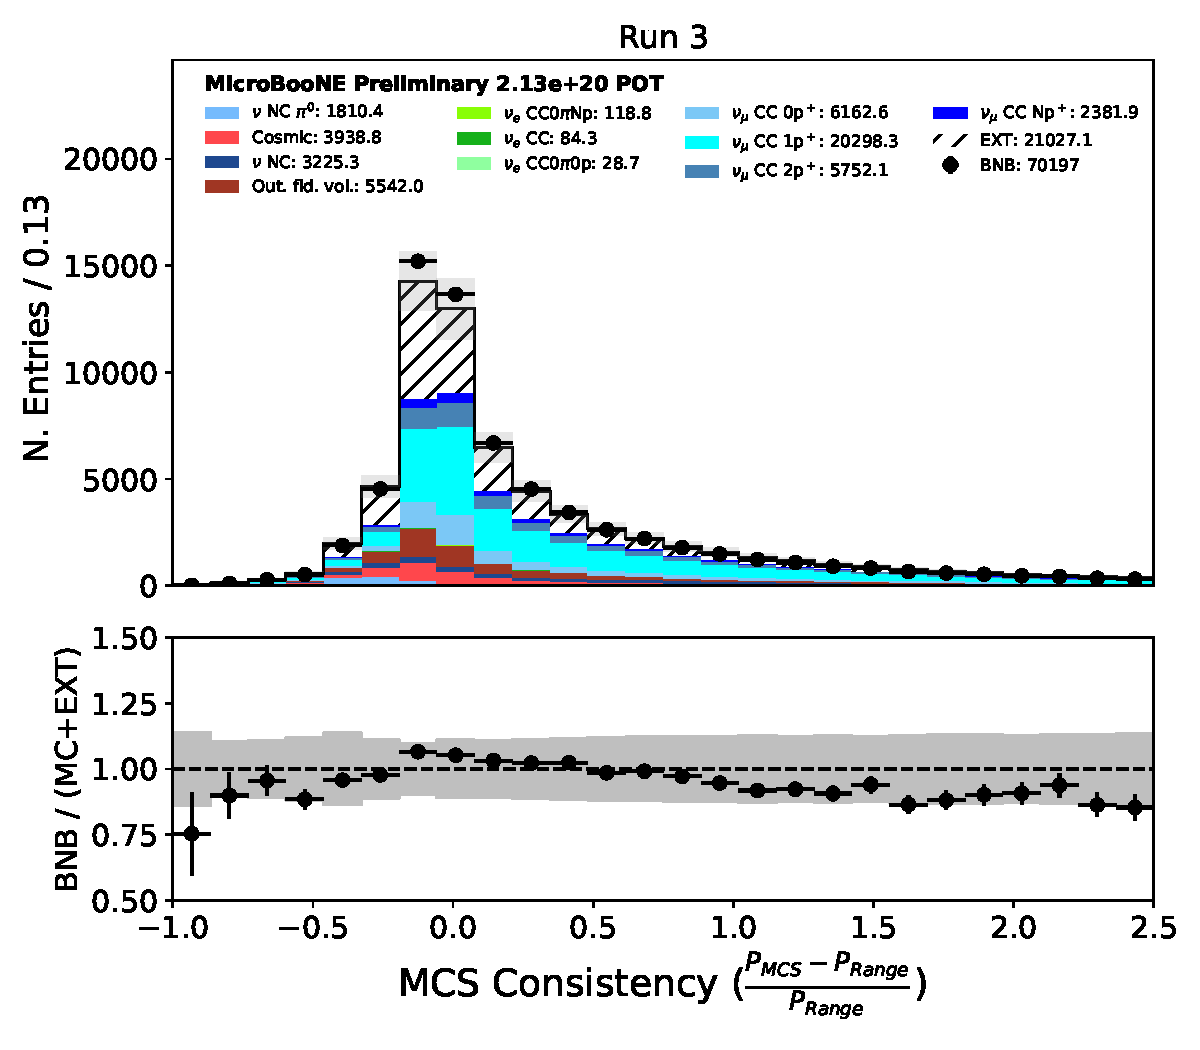
\includegraphics[width=1.00\textwidth]{NuMuCCsel/Images/Ryan/Run3_nocrt/trk_p_quality_v_08052020_presel_samples_longest_noCRT_event_category.pdf}
    \end{subfigure} %\newline
    \begin{subfigure}[b]{0.35\textwidth}
        \centering
        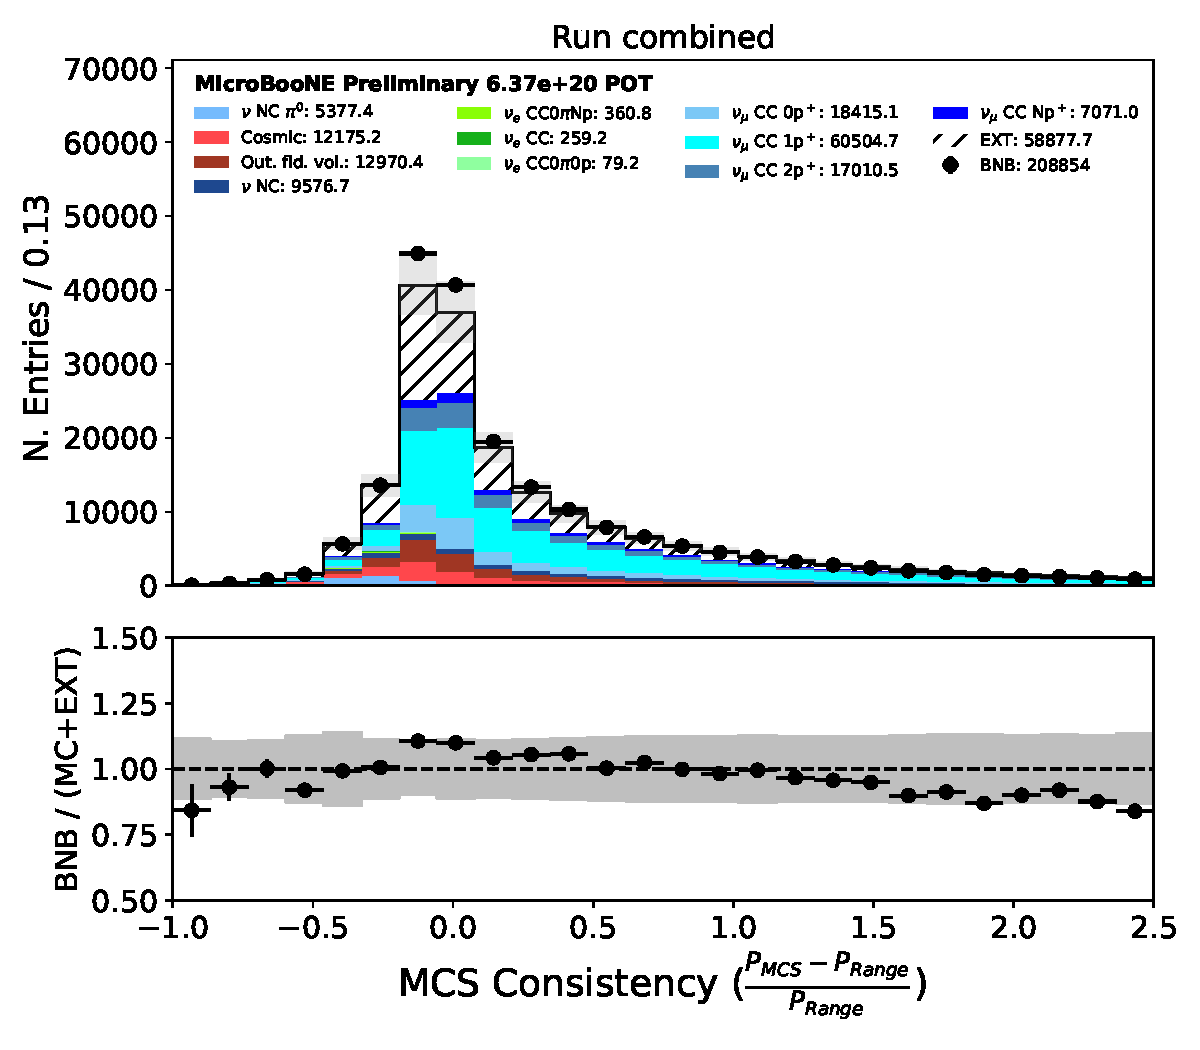
\includegraphics[width=1.00\textwidth]{NuMuCCsel/Images/Ryan/combined/trk_p_quality_v_08052020_presel_samples_longest_noCRT_event_category.pdf}
    \end{subfigure}
\caption{Time dependence of MCS consistency variable for muon candidates after preselection.}
\label{fig:NuMuCCsel:timedep:MCSquality}
\end{center}
\end{figure}

\begin{figure}[hbt!] 
\begin{center}
    \begin{subfigure}[b]{0.35\textwidth}
        \centering
        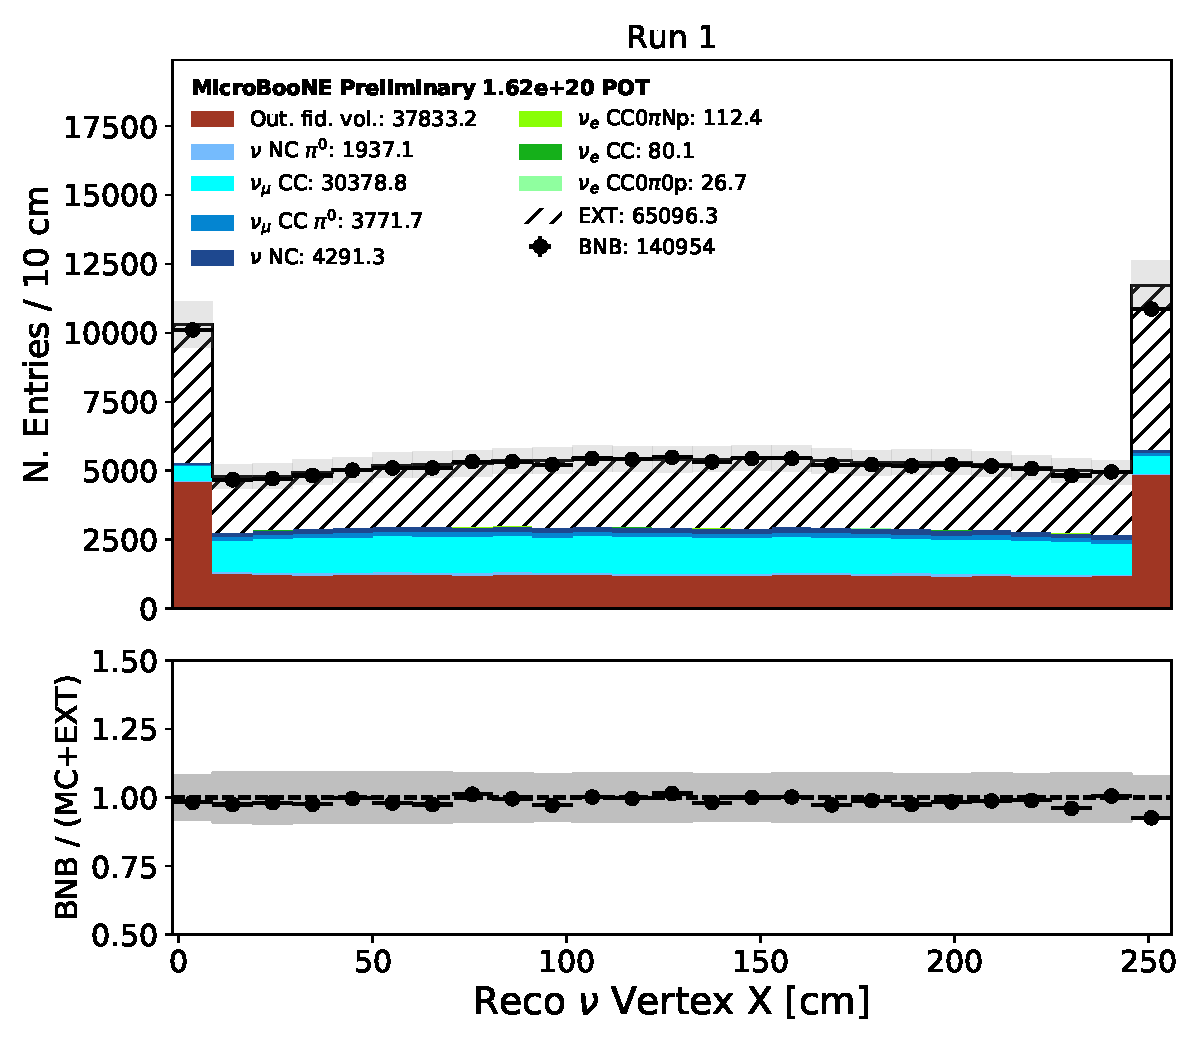
\includegraphics[width=1.00\textwidth]{NuMuCCsel/Images/Ryan/Run1/reco_nu_vtx_sce_x_08062020_samples_longest_noCRT_event_category.pdf}
    \end{subfigure}
    \begin{subfigure}[b]{0.35\textwidth}
        \centering
        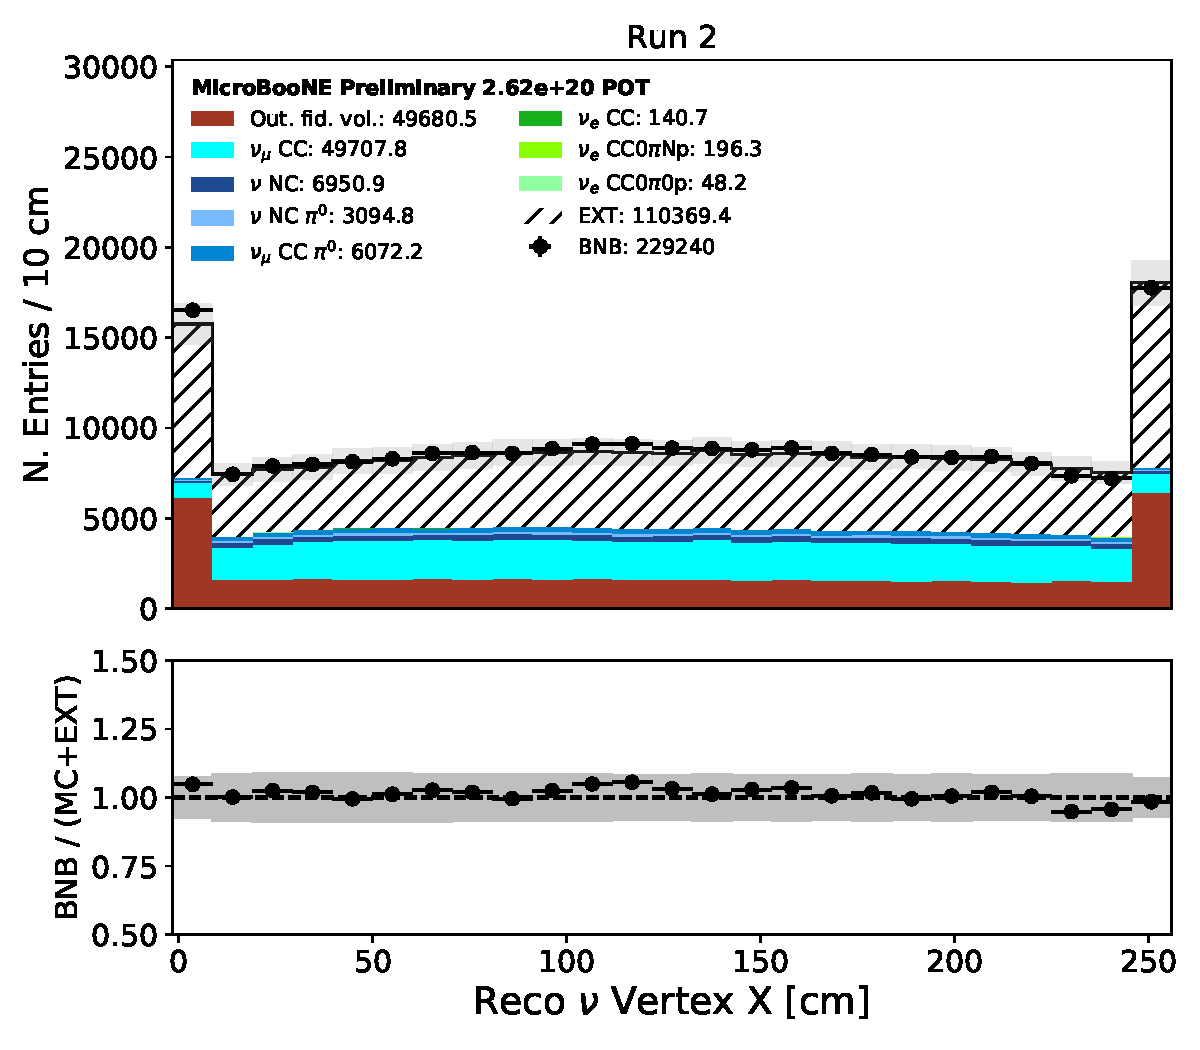
\includegraphics[width=1.00\textwidth]{NuMuCCsel/Images/Ryan/Run2/reco_nu_vtx_sce_x_08062020_samples_longest_noCRT_event_category.pdf}
    \end{subfigure}
    \begin{subfigure}[b]{0.35\textwidth}
        \centering
        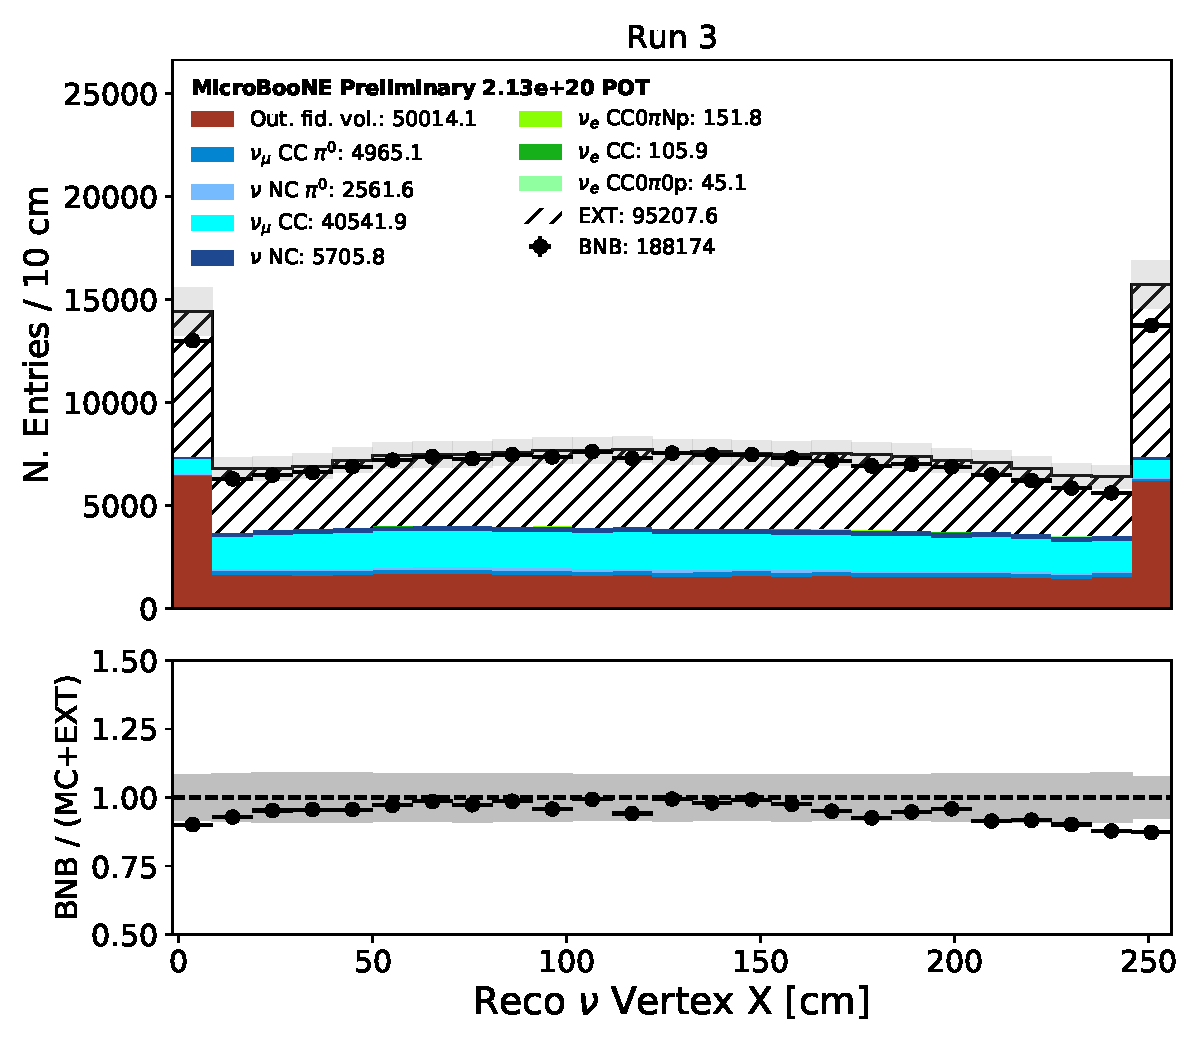
\includegraphics[width=1.00\textwidth]{NuMuCCsel/Images/Ryan/Run3_nocrt/reco_nu_vtx_sce_x_08062020_samples_longest_noCRT_event_category.pdf}
    \end{subfigure} %\newline
\caption{Time dependence of X coordinate of reconstructed vertex position. Only SliceID applied.}
\label{fig:NuMuCCsel:timedep:vtxX}
\end{center}
\end{figure}

\begin{figure}[hbt!] 
\begin{center}
    \begin{subfigure}[b]{0.35\textwidth}
        \centering
        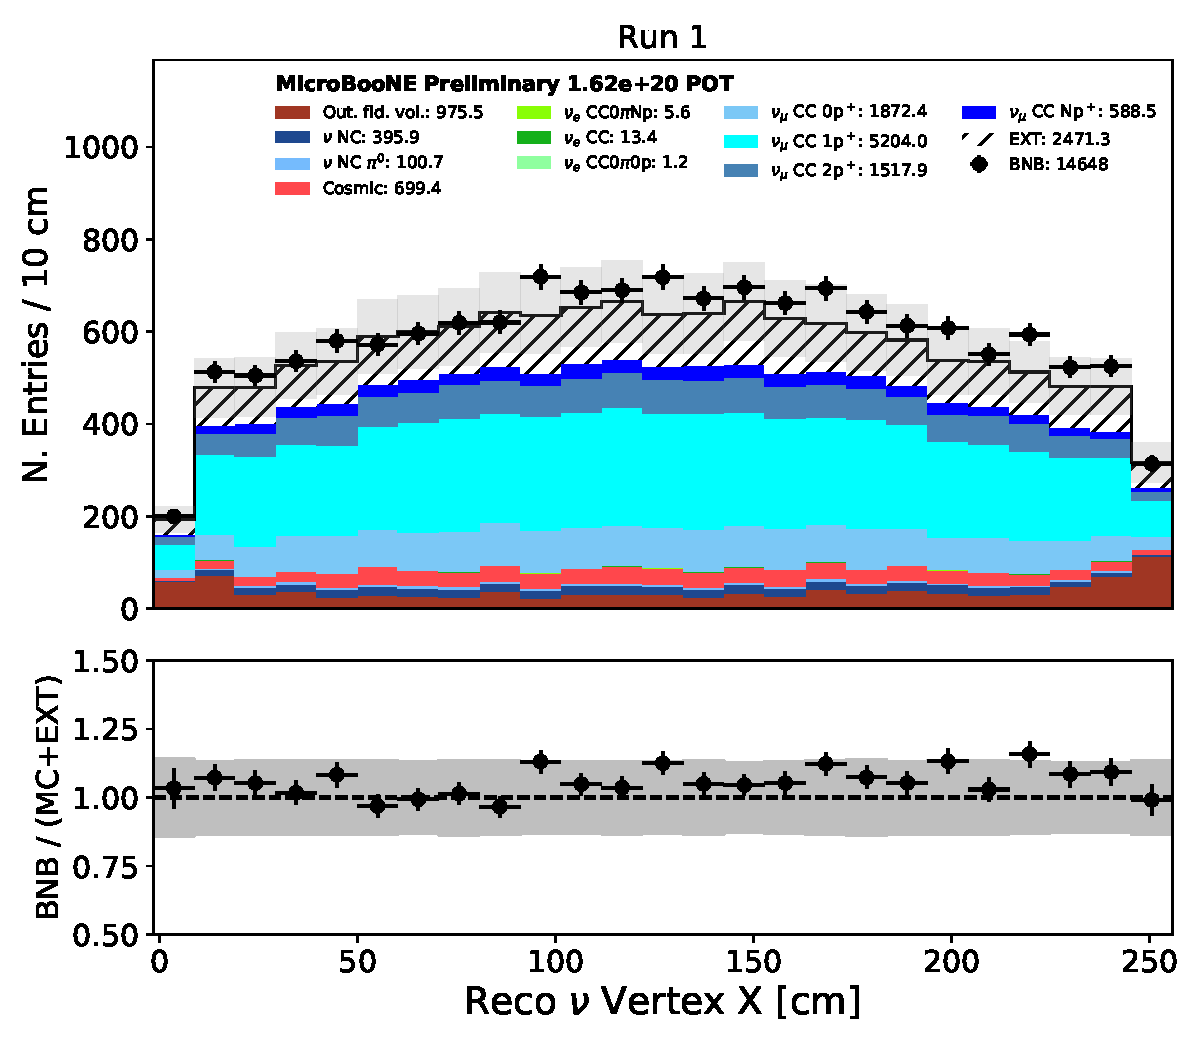
\includegraphics[width=1.00\textwidth]{NuMuCCsel/Images/Ryan/Run1/reco_nu_vtx_sce_x_08072020_fullsel_samples_longest_noCRT_event_category.pdf}
    \end{subfigure}
    \begin{subfigure}[b]{0.35\textwidth}
        \centering
        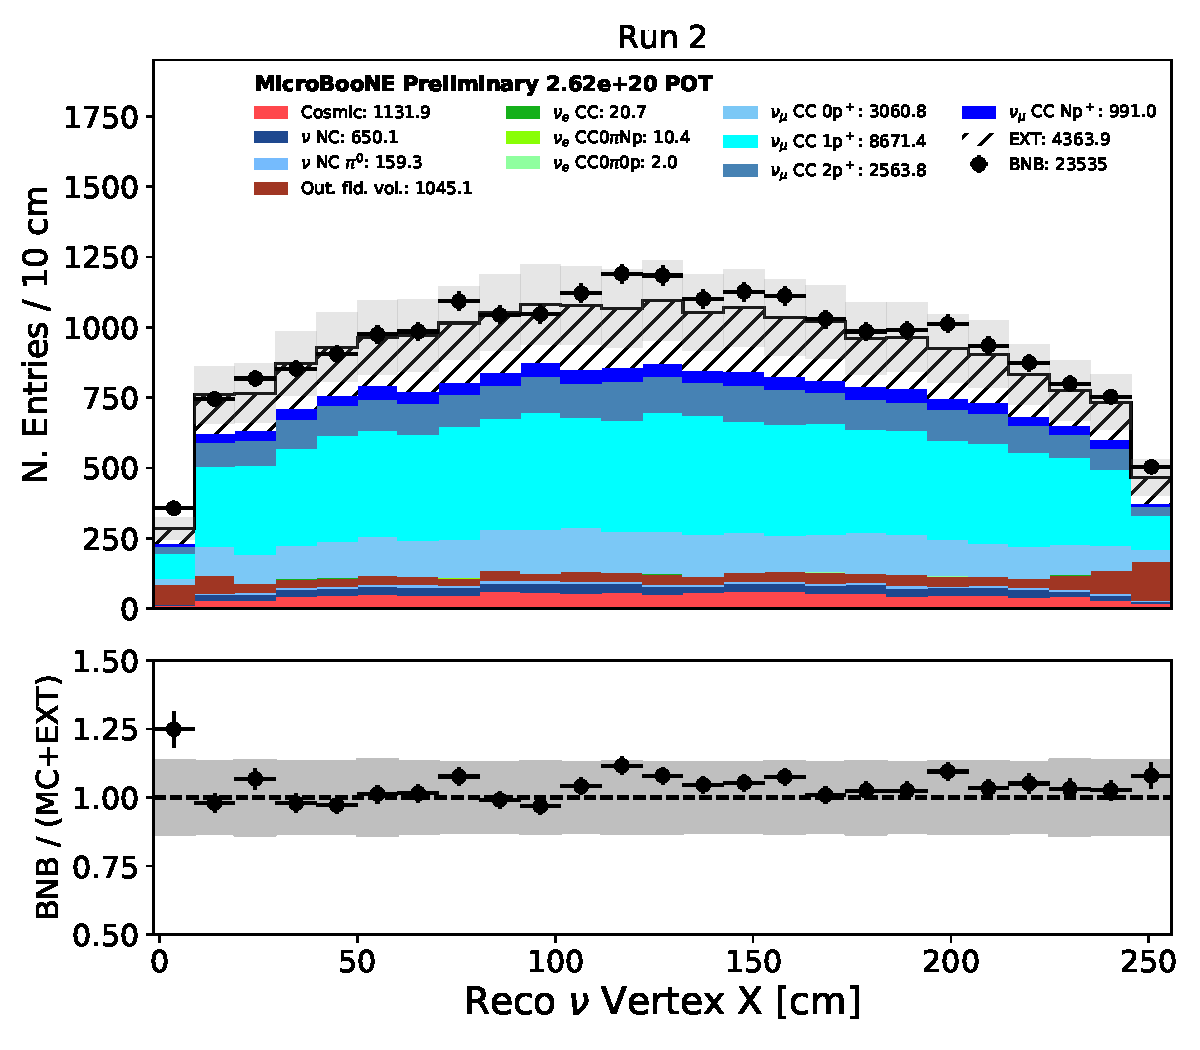
\includegraphics[width=1.00\textwidth]{NuMuCCsel/Images/Ryan/Run2/reco_nu_vtx_sce_x_08072020_fullsel_samples_longest_noCRT_event_category.pdf}
    \end{subfigure}
    \begin{subfigure}[b]{0.35\textwidth}
        \centering
        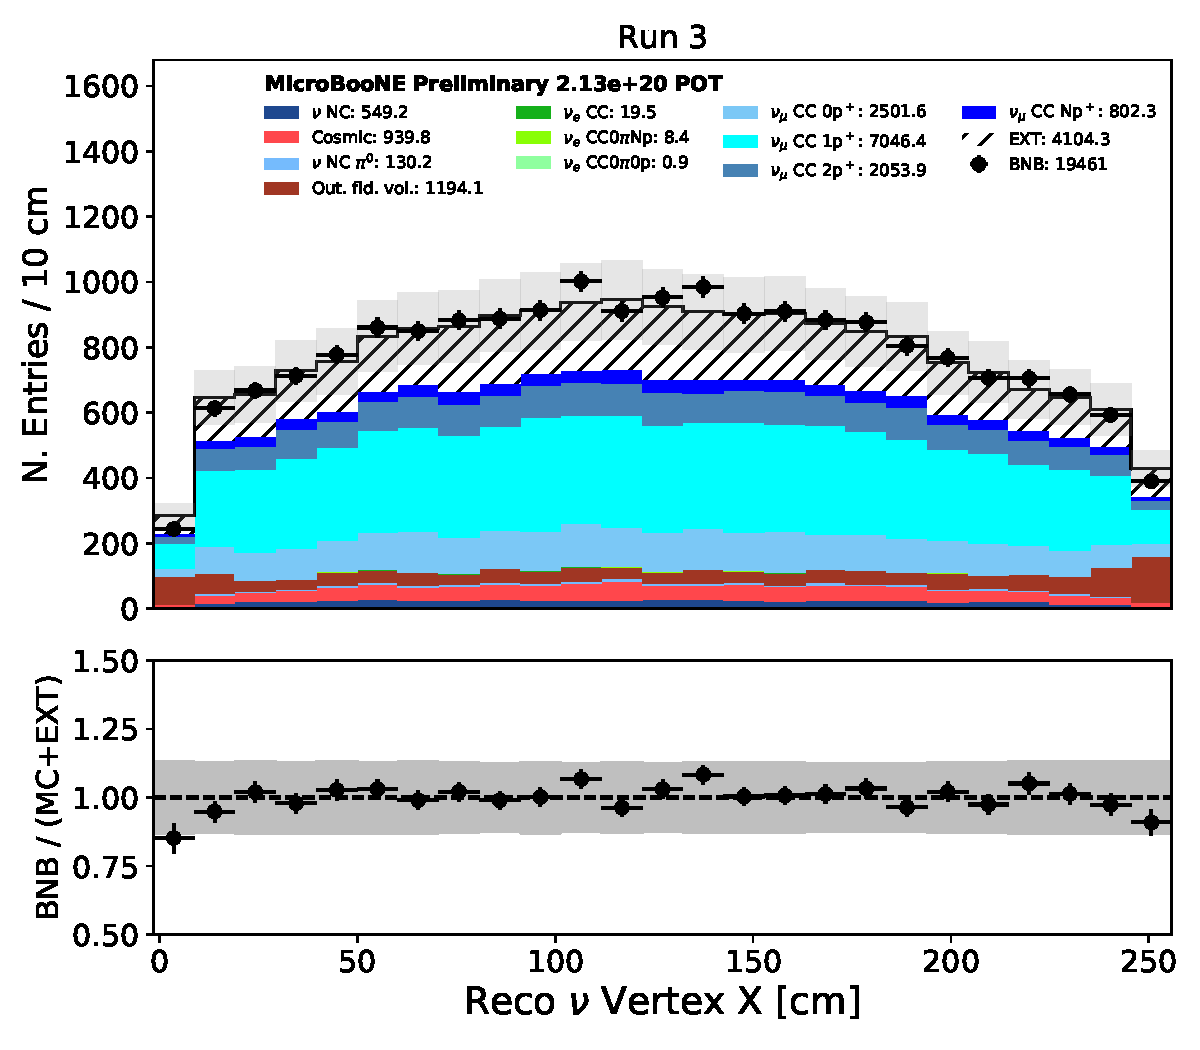
\includegraphics[width=1.00\textwidth]{NuMuCCsel/Images/Ryan/Run3_nocrt/reco_nu_vtx_sce_x_08072020_fullsel_samples_longest_noCRT_event_category.pdf}
    \end{subfigure} %\newline
\caption{Time dependence of X coordinate of reconstructed vertex position. Full selection applied.}
\label{fig:NuMuCCsel:timedep:vtxX_fullsel}
\end{center}
\end{figure}

\begin{figure}[hbt!] 
\begin{center}
    \begin{subfigure}[b]{0.35\textwidth}
        \centering
        \includegraphics[width=1.00\textwidth]{NuMuCCsel/Images/Ryan/Run1/topological_score_08062020_samples_longest_noCRT_event_category.pdf}
    \end{subfigure}
    \begin{subfigure}[b]{0.35\textwidth}
        \centering
        \includegraphics[width=1.00\textwidth]{NuMuCCsel/Images/Ryan/Run2/topological_score_08062020_samples_longest_noCRT_event_category.pdf}
    \end{subfigure}
    \begin{subfigure}[b]{0.35\textwidth}
        \centering
        \includegraphics[width=1.00\textwidth]{NuMuCCsel/Images/Ryan/Run3_nocrt/topological_score_08062020_samples_longest_noCRT_event_category.pdf}
    \end{subfigure} %\newline
\caption{Time dependence of topological score. Only SliceID applied.}
\label{fig:NuMuCCsel:timedep:topo}
\end{center}
\end{figure}

\begin{figure}[hbt!] 
\begin{center}
    \begin{subfigure}[b]{0.35\textwidth}
        \centering
        \includegraphics[width=1.00\textwidth]{NuMuCCsel/Images/Ryan/Run1/topological_score_08072020_fullsel_samples_longest_noCRT_event_category.pdf}
    \end{subfigure}
    \begin{subfigure}[b]{0.35\textwidth}
        \centering
        \includegraphics[width=1.00\textwidth]{NuMuCCsel/Images/Ryan/Run2/topological_score_08072020_fullsel_samples_longest_noCRT_event_category.pdf}
    \end{subfigure}
    \begin{subfigure}[b]{0.35\textwidth}
        \centering
        \includegraphics[width=1.00\textwidth]{NuMuCCsel/Images/Ryan/Run3_nocrt/topological_score_08072020_fullsel_samples_longest_noCRT_event_category.pdf}
    \end{subfigure} %\newline
\caption{Time dependence of topological score. Full selection applied.}
\label{fig:NuMuCCsel:timedep:topo_fullsel}
\end{center}
\end{figure}

\begin{figure}[hbt!]
    \centering
    \includegraphics[width=0.5\linewidth]{NuMuCCsel/Images/Ryan/other/RUN_SPECTRUM.PNG}
    \caption{Number of events collected as a function of event number. Each bin represents several weeks.}
    \label{fig:NuMuCCsel:timedep:RunsDistribution}
\end{figure}